\documentclass[ALICE,manyauthors]{cernphprep}
\usepackage[comma,square,numbers,sort&compress]{natbib}
\usepackage{hyperref}
\usepackage{lineno}
\usepackage{xspace}
\usepackage[table]{xcolor}
\usepackage{siunitx}
\sisetup{binary-units=true}
\sisetup{load-configurations = abbreviations}
\linenumbers

%%%%%%%%%%%%%%%%%%%%%%%%%%%%%%%%%%%%%%%%%%%%%%%%%%
% These are some new commands that may be useful 
% for paper writing in general. If other newcommands
% are needed for your specific paper, please feel 
% free to add here. 
%
% The currently available commands are organized in: 
% 1) Systems
% 2) Quantities
% 3) Energies and units
% 4) Detectors
% 5) particle species 
%%%%%%%%%%%%%%%%%%%%%%%%%%%%%%%%%%%%%%%%%%%%%%%%%%

% 1) SYSTEMS 
\newcommand{\pp}           {pp\xspace}
\newcommand{\ppbar}        {\mbox{$\mathrm {p\overline{p}}$}\xspace}
\newcommand{\XeXe}         {\mbox{Xe--Xe}\xspace}
\newcommand{\PbPb}         {\mbox{Pb--Pb}\xspace}
\newcommand{\pA}           {\mbox{pA}\xspace}
\newcommand{\pPb}          {\mbox{p--Pb}\xspace}
\newcommand{\AuAu}         {\mbox{Au--Au}\xspace}
\newcommand{\dAu}          {\mbox{d--Au}\xspace}

% 2) QUANTITIES 
\newcommand{\s}            {\ensuremath{\sqrt{s}}\xspace}
\newcommand{\snn}          {\ensuremath{\sqrt{s_{\mathrm{NN}}}}\xspace}
\newcommand{\pt}           {\ensuremath{p_{\rm T}}\xspace}
\newcommand{\meanpt}       {$\langle p_{\mathrm{T}}\rangle$\xspace}
\newcommand{\ycms}         {\ensuremath{y_{\rm CMS}}\xspace}
\newcommand{\ylab}         {\ensuremath{y_{\rm lab}}\xspace}
\newcommand{\etarange}[1]  {\mbox{$\left | \eta \right |~<~#1$}}
\newcommand{\yrange}[1]    {\mbox{$\left | y \right |~<~#1$}}
\newcommand{\dndy}         {\ensuremath{\mathrm{d}N_\mathrm{ch}/\mathrm{d}y}\xspace}
\newcommand{\dndeta}       {\ensuremath{\mathrm{d}N_\mathrm{ch}/\mathrm{d}\eta}\xspace}
\newcommand{\avdndeta}     {\ensuremath{\langle\dndeta\rangle}\xspace}
\newcommand{\dNdy}         {\ensuremath{\mathrm{d}N_\mathrm{ch}/\mathrm{d}y}\xspace}
\newcommand{\Npart}        {\ensuremath{N_\mathrm{part}}\xspace}
\newcommand{\Ncoll}        {\ensuremath{N_\mathrm{coll}}\xspace}
\newcommand{\dEdx}         {\ensuremath{\textrm{d}E/\textrm{d}x}\xspace}
\newcommand{\RpPb}         {\ensuremath{R_{\rm pPb}}\xspace}

% 3) ENERGIES, UNITS
\newcommand{\nineH}        {$\sqrt{s}~=~0.9$~Te\kern-.1emV\xspace}
\newcommand{\seven}        {$\sqrt{s}~=~7$~Te\kern-.1emV\xspace}
\newcommand{\twoH}         {$\sqrt{s}~=~0.2$~Te\kern-.1emV\xspace}
\newcommand{\twosevensix}  {$\sqrt{s}~=~2.76$~Te\kern-.1emV\xspace}
\newcommand{\five}         {$\sqrt{s}~=~5.02$~Te\kern-.1emV\xspace}
\newcommand{\twosevensixnn}{$\sqrt{s_{\mathrm{NN}}}~=~2.76$~Te\kern-.1emV\xspace}
\newcommand{\fivenn}       {$\sqrt{s_{\mathrm{NN}}}~=~5.02$~Te\kern-.1emV\xspace}
\newcommand{\LT}           {L{\'e}vy-Tsallis\xspace}
\newcommand{\GeVc}         {Ge\kern-.1emV/$c$\xspace}
\newcommand{\MeVc}         {Me\kern-.1emV/$c$\xspace}
\newcommand{\TeV}          {Te\kern-.1emV\xspace}
\newcommand{\GeV}          {Ge\kern-.1emV\xspace}
\newcommand{\MeV}          {Me\kern-.1emV\xspace}
\newcommand{\GeVmass}      {Ge\kern-.2emV/$c^2$\xspace}
\newcommand{\MeVmass}      {Me\kern-.2emV/$c^2$\xspace}
\newcommand{\lumi}         {\ensuremath{\mathcal{L}}\xspace}

% 4) DETECTORS 
\newcommand{\ITS}          {\rm{ITS}\xspace}
\newcommand{\TOF}          {\rm{TOF}\xspace}
\newcommand{\ZDC}          {\rm{ZDC}\xspace}
\newcommand{\ZDCs}         {\rm{ZDCs}\xspace}
\newcommand{\ZNA}          {\rm{ZNA}\xspace}
\newcommand{\ZNC}          {\rm{ZNC}\xspace}
\newcommand{\SPD}          {\rm{SPD}\xspace}
\newcommand{\SDD}          {\rm{SDD}\xspace}
\newcommand{\SSD}          {\rm{SSD}\xspace}
\newcommand{\TPC}          {\rm{TPC}\xspace}
\newcommand{\TRD}          {\rm{TRD}\xspace}
\newcommand{\VZERO}        {\rm{V0}\xspace}
\newcommand{\VZEROA}       {\rm{V0A}\xspace}
\newcommand{\VZEROC}       {\rm{V0C}\xspace}
\newcommand{\Vdecay} 	   {\ensuremath{V^{0}}\xspace}

% 4) PARTICLE SPECIES 
\newcommand{\ee}           {\ensuremath{e^{+}e^{-}}} 
\newcommand{\pip}          {\ensuremath{\pi^{+}}\xspace}
\newcommand{\pim}          {\ensuremath{\pi^{-}}\xspace}
\newcommand{\kap}          {\ensuremath{\rm{K}^{+}}\xspace}
\newcommand{\kam}          {\ensuremath{\rm{K}^{-}}\xspace}
\newcommand{\pbar}         {\ensuremath{\rm\overline{p}}\xspace}
\newcommand{\kzero}        {\ensuremath{{\rm K}^{0}_{\rm{S}}}\xspace}
\newcommand{\lmb}          {\ensuremath{\Lambda}\xspace}
\newcommand{\almb}         {\ensuremath{\overline{\Lambda}}\xspace}
\newcommand{\Om}           {\ensuremath{\Omega^-}\xspace}
\newcommand{\Mo}           {\ensuremath{\overline{\Omega}^+}\xspace}
\newcommand{\X}            {\ensuremath{\Xi^-}\xspace}
\newcommand{\Ix}           {\ensuremath{\overline{\Xi}^+}\xspace}
\newcommand{\Xis}          {\ensuremath{\Xi^{\pm}}\xspace}
\newcommand{\Oms}          {\ensuremath{\Omega^{\pm}}\xspace}
\newcommand{\degree}       {\ensuremath{^{\rm o}}\xspace}

\begin{document}

\begin{titlepage}
% the dates below correspond to CERN approval
% please don't touch: EB chairs will take care
\PHyear{XXXX}       % required, will be obtained from CERN
\PHnumber{XXX}      % required, will be obtained from CERN
\PHdate{Day Month}  % required, will be obtained from CERN

%%% Put your own title + short title here:
\title{ALICE upgrades during the LHC long-shutdown 2}
\ShortTitle{ALICE LS2 upgrades}   % appears on left page headers

%%% Do not change the next lines
\Collaboration{ALICE Collaboration\thanks{See Appendix~\ref{app:collab} for the list of collaboration members}}
\ShortAuthor{ALICE Collaboration} % appears on right page headers, do not change

\begin{abstract}
A Large Ion Collider Experiment (ALICE) has been conceived and constructed as a heavy-ion experiment at the LHC. During LHC runs 1 and 2, it has produced a wide range of physics results based using all collision systems available at the LHC.
In order to best exploit new physics opportunities opening up with the upgraded LHC and new detector technologies, the experiment has undergone a major upgrade during the LHC long shutdown 2. This comprises the move to continuous read-out, the complete overhaul of core detectors, as well as a new processing software stack and hardware. 
These improvements will allow us to sample Pb-Pb collisions at rates up to 50 kHz, while ensuring sensitivity for signals without a triggerable signature.
\end{abstract}
\end{titlepage}

\setcounter{page}{2} %please do not remove this line

\tableofcontents
\listoffigures
\listoftables

\section{Introduction (Marco, Jochen; 8 p.)}

A Large Ion Collider Experiment (ALICE) has been proposed and built to study
the properties of the Quark-Gluon Plasma in hadronic collisions at the Large
Hadron Collider at CERN~\cite{Aamodt:2008zz}. The design was driven by the
requirement to cope with the high multiplicities in central \PbPb collisions
and provide a complete reconstruction of the events, including particle
identification over a wide \pt range.

The experimental setup consists of a central barrel contained in a solenoidal
magnet ($B = 0.5~\mathrm{Tesla}$) and a forward muon-system with a dipole magnet
providing $3~\mathrm{Tm}$, see Fig.~\ref{fig:alice_run2}. Until the end of Run~2,
the central barrel contained an Inner Tracking System (ITS) with two layers of
Silicon Pixel Detectors (SPD), two layers of Silicon Drift Detectors (SDD), and
two layers of Silicon Strip Detectors (SSD). In radial direction, it is followed
by a Time Projection Chamber (TPC) covering the radii from 0.5~m to 2.5~m over a
length of 7~m.
The central barrel detector system is designed for efficient trakcing in the high track-density environment of heavy ion collisions, covering momenta from low to high \pt{} with good hadron and electron identification capabilities.

The forward muon detectors cover the rapidity range $2.5 < \eta < 4.0$ (tbc) and use a system of absobers to remove hadrons and idensify muons.
The background of secondary muons from pion and kaon decays in the muon system is small at high pt, thanks to the so-called 'muon plug' absorber, which is placed at $z = xx$ cm from the interaction point.

The forward muon detectors cover the rapidity range $2.5 < \eta < 4.0$ (tbc) and use a system of absobers to remove hadrons and idensify muons.
The background of secondary muons from pion and kaon decays in the muon system is small at high pt, thanks to the so-called 'muon plug' absorber, which is placed at $z = xx$ cm from the interaction point.

\subsection{Tracking}

The ALICE detector system is designed for high-efficiency tracking with excellent two-track separation in high-multiplicity events. The efficient tracking extends down to low $\pt \approx \SI{100}{\mega\eV\per\clight}$ (todo: check canonical value) which is important to access the kinematic range where thermal production from the QGP plays a role and to reconstruct weak and strong decays.
Similarly, the two-track resolution is important for decay reconstruction, as well as correlation measurements that reveal the space-time structure of particle production ('femtoscopy') and probe interactions between hadrons as well as jet structure measurements.

Give some key performance numbers: momentum resolution and impact parameter resolution...

\subsection{Tracking performance}

The ALICE detector system is designed for high-efficiency tracking with excellent two-track separation in high-multiplicity events. The efficient tracking extends down to low $\pt \approx 100$ MeV/$c$ (todo: check canonical value) which is important to access the kinematic range where thermal production from the QGP plays a role and to reconstruct weak and strong decays.
Similarly, the two-track resolution is important for decay reconstruction, as well as correlation measurements that reveal the space-time structure of particle production ('femtoscopy') and probe interactions between hadrons as well as jet structure measurements.

Give some key performance numbers: momentum resolution and impact parameter resolution...

\begin{figure}
\centering
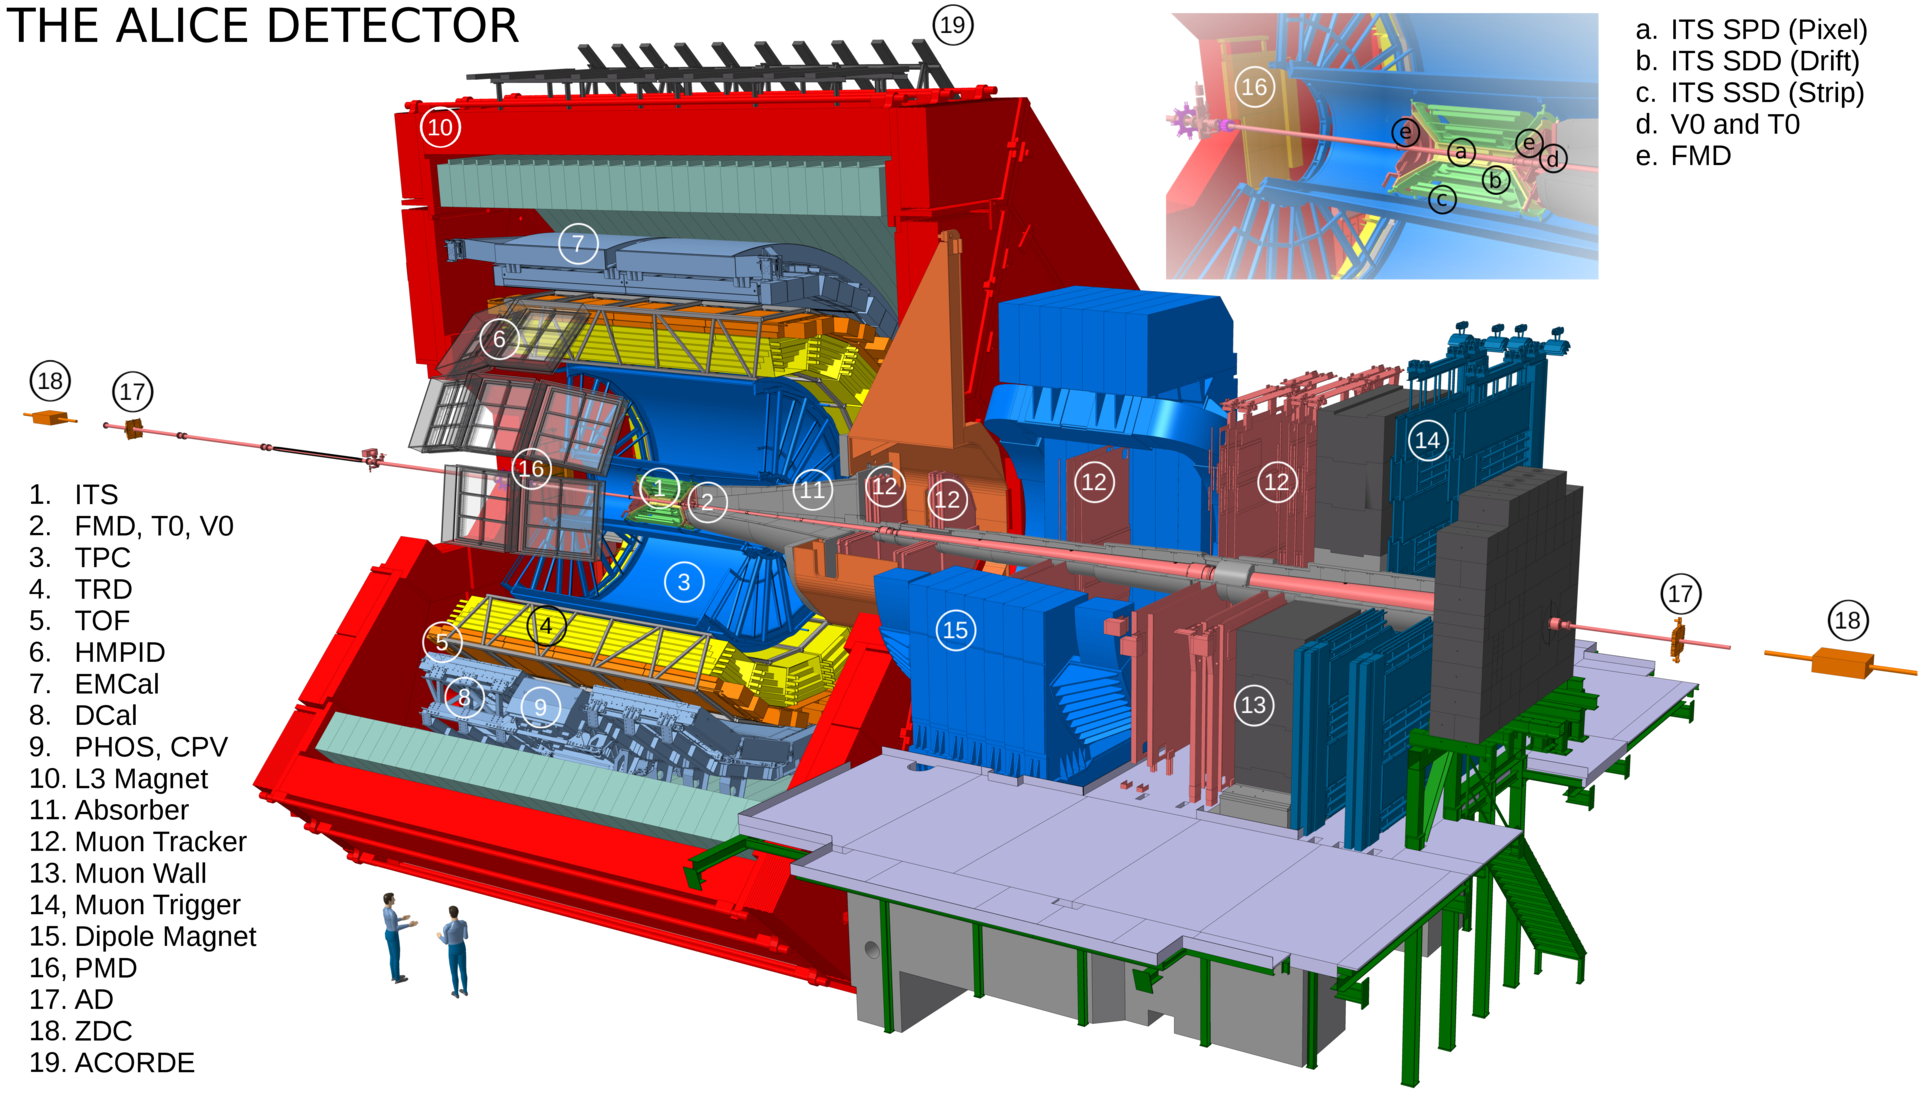
\includegraphics[width=.7\textwidth]{intro/2017-May-11-ALICE_RUN2_labels_HD}
\caption{Detector setup in Run 2}
\label{fig:alice_run2}
\end{figure}

\begin{figure}
\centering
\caption{tracking efficiency}
\label{fig:trk_eff}
\end{figure}

\begin{figure}
\centering
\caption{tracking \pt resolution}
\label{fig:trk_res}
\end{figure}

\subsection{Calorimetry}

\subsection{Particle identification}

\begin{figure}
\centering
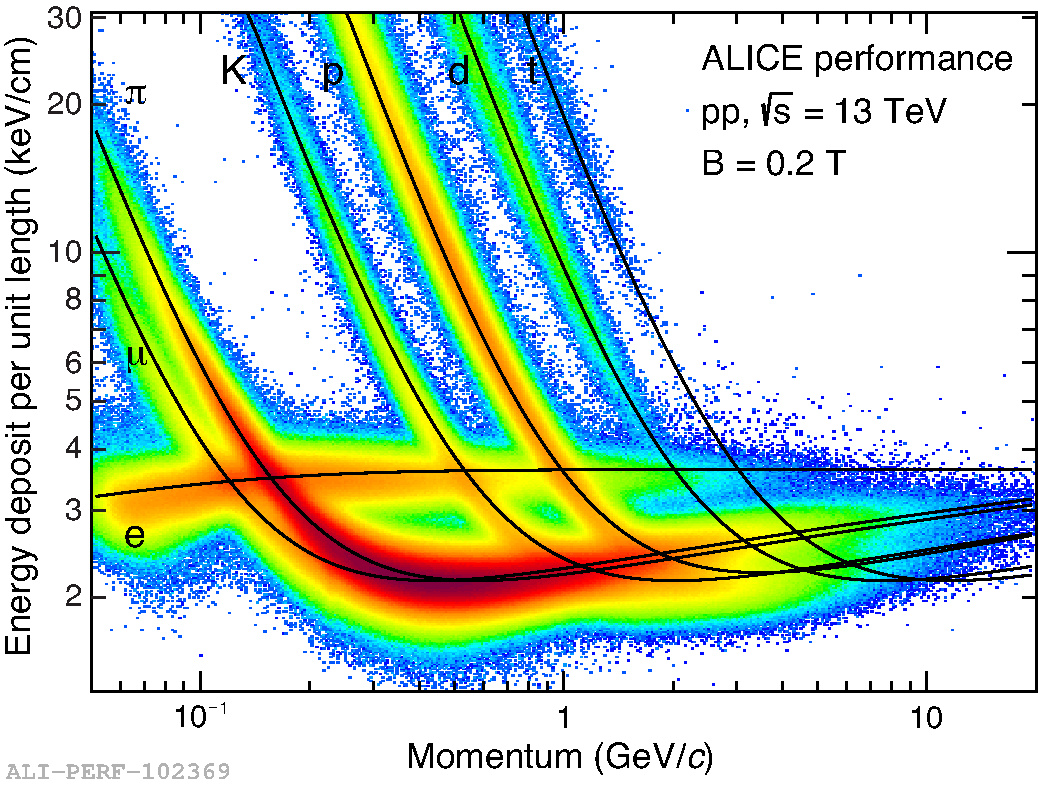
\includegraphics[width=.7\textwidth]{intro/2018-Jul-23-TPC_dEdx_2T_151003_color}
\caption{TPC dE/dx}
\label{fig:tpc_dedx}
\end{figure}

\subsection{Event characterization and selection}

\subsection{Forward spectrometer}

\subsection*{Run1/2 performance highlights (examples)}

cite performance paper~\cite{Abelev:2014ffa}, possibly also detector papers

discuss performance
\begin{itemize}
\item particle identification and relevant detectors
\item secondary vertex resolution
\item data sets (rate/integrated luminosity)
\end{itemize}

Data was recorded throughout the
running of the LHC in Run 1 and 2 exploiting a variety of collision systems and
energies, see Tab.~\ref{tab:datasets}.

\begin{figure}
\centering
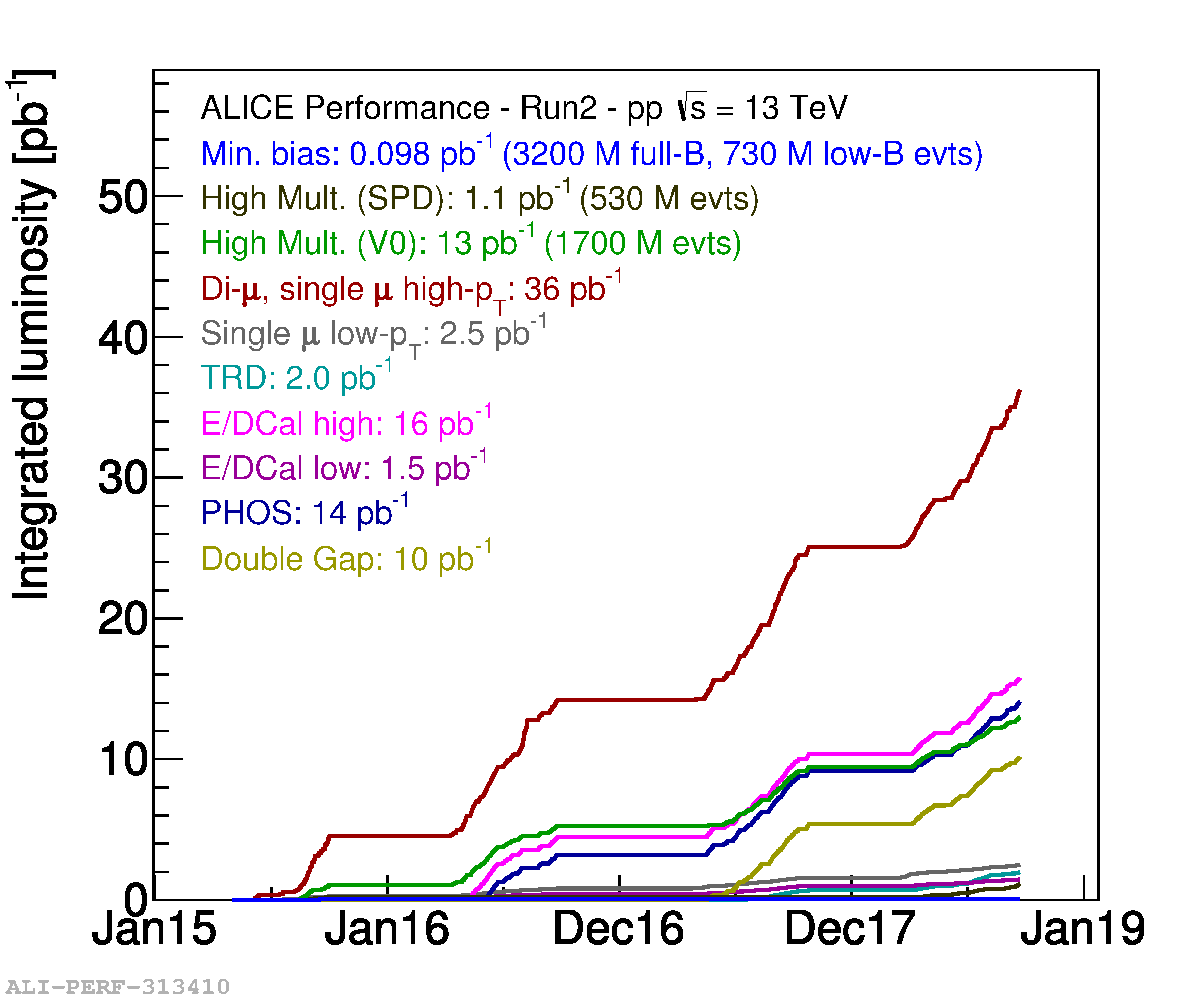
\includegraphics[width=.45\textwidth]{intro/2019-01-17-2019-01-17-lumi_Run2_pp13TeV}
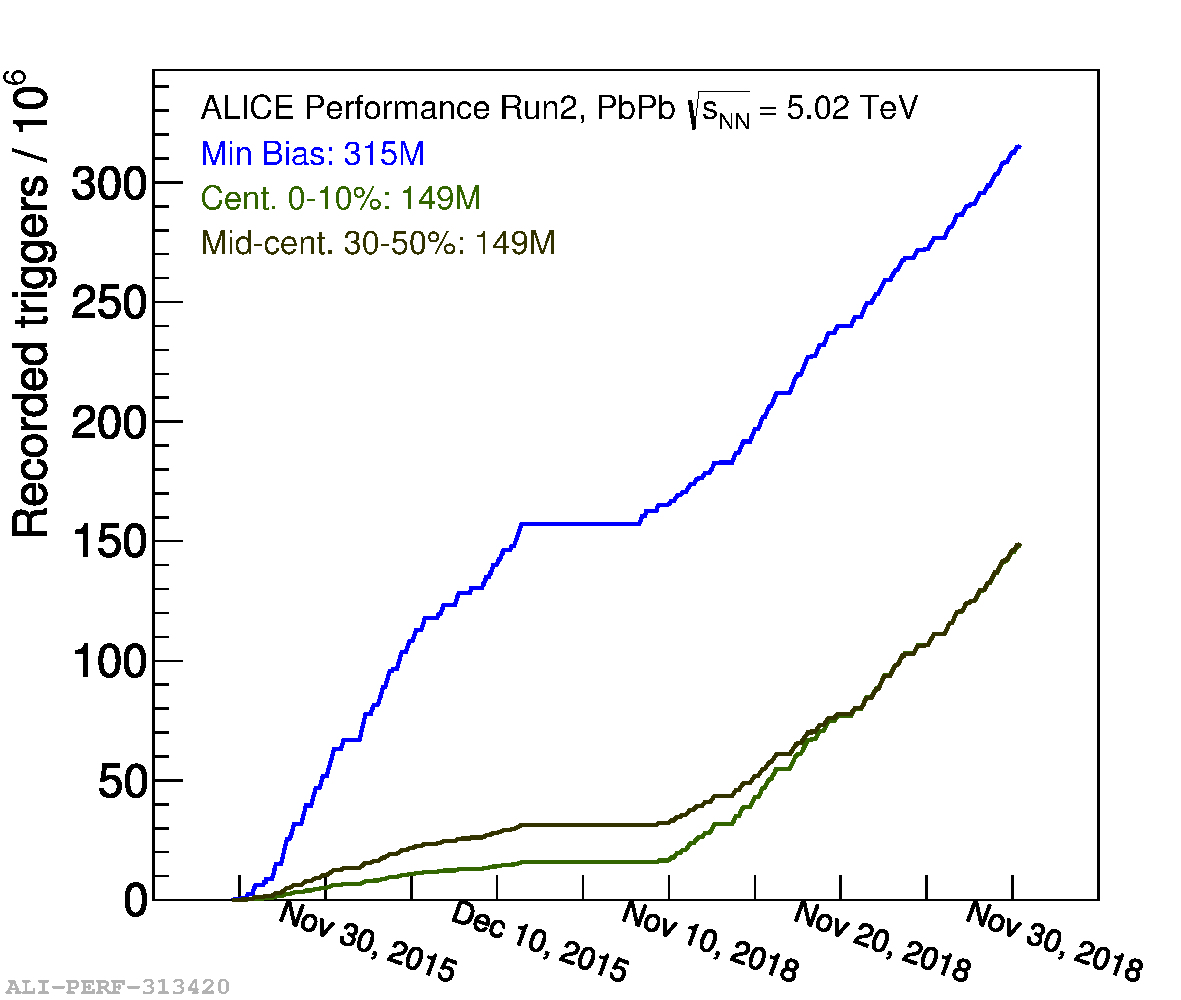
\includegraphics[width=.45\textwidth]{intro/2019-01-17-2019-01-17-stat_Run2_PbPb}
\caption{integrated lumi}
\label{fig:lumi_run2}
\end{figure}

\begin{table}
  \centering
  \begin{tabular}{lrrr}
    \multicolumn{1}{c}{system}
    & \multicolumn{1}{c}{$\snn~(\mathrm{\TeV})$}
    & \multicolumn{1}{c}{$L_\mathrm{MB}$}
    & \multicolumn{1}{c}{$L_\mathrm{insp}$}\\
    \hline \hline
    \pp & 0.9 & & $\sim \SI{200}{\micro \barn^{-1}}$\\
        & 2.76 & & $\sim 100~\mathrm{nb}^{-1}$\\
        & 5.02 & & $\sim 1.3~\mathrm{pb}^{-1}$\\
        & 7 & & $\sim 1.5~\mathrm{pb}^{-1}$\\
        & 8 & & $\sim 2.5~\mathrm{pb}^{-1}$\\
        & 13 & & $\sim 25~\mathrm{pb}^{-1}$\\
    \pPb{} & 5.02 & & $\sim 15 + 3~\mathrm{nb}^{-1}$\\
           & 8.16 & & $\sim 25~\mathrm{nb}^{-1}$\\
    \XeXe{} & 5.44 & & $\sim 0.3~\mu\mathrm{b}^{-1}$\\
    \PbPb{} & 2.76 & & $\sim 75~\mu\mathrm{b}^{-1}$\\
            & 5.02 & & $\sim 0.25 + 1~\mathrm{nb}^{-1}$\\
    \hline
  \end{tabular}
  \caption{ALICE datasets from LHC Run 1 and 2}
  \label{tab:datasets}
\end{table}


\section{Upgrade objectives, motivations and goals (10 p.)}

The ALICE detector has undergone a major upgrade during the Long Shutdown 2 of the LHC, 2019-2021.
The main goal of the upgrade is to improve the performance for rare, untriggered signals: the production of open heavy flavor mesons and baryons which serve as important 'trace particles' that probe both early and late time dynamics in the collision, as well as electron-positron pairs which measure the temperature of the hot and dense Quark Gluon Plasma produced in the collision, as well as effects related to chiral symmetry restoration.
To achieve this, the full Inner Tracking System has been replaced with a new system based on monolithic active pixel sensors with a better spatial resolution than the previous ITS, as well as a lower material budget, to further improve the spatial resolution and reduce the background from photon conversions. The readout chambers of the TPC have been replaced with multi-foil GEM chambers to reduce the ion backflow and allow continuous readout of the TPC.
In the forward direction, the new Muon Forward Tracker (MFT) is a silicon pixel tracker that provides accurate pointing for muon tracks, to identify quarkonia from beauty decays.
The trigger and data acquisition systems have been completely redesigned and replaced with an online processing system that performs important parts of the reconstruction, to reduce the data rate while keeping information on all events and primary tracks. The readout electronics of several sub-detectors has been replaced to provide larger readout rates than were previously possible and to be compatible with the new online data acquisition and processing system. 

\subsection{Physics performance (Marco, Jochen)}

The physics programme motivating the upgrade was first established in the Letter of Intent~\cite{Abelevetal:2014cna} and the individual Technical Design Reports. Later, it was scrutinized by Working Group 5 of \dots leading to a report~\cite{Citron:2018lsq}, which summarizes the potential of heavy-ion physics at the LHC in Run 3 and 4 across all the LHC experiments. This report identified core areas of interests and the corresponding measurements and observables. The precise measurement of the long-wavelength behaviour, i.e. the macroscopic fluid-like evolution of a high-density and high-temperature system, allows us to draw conclusions on the phase transition as well as material properties of a deconfined state of matter. Access to the microscopic parton dynamics which underlies the QGP allows us to understand the fundamental degrees of freedom and interactions in a deconfined state. A further goal is to systematicaly study particle production across collision systems in order to assess the validity of the fluid description and the role of collectivity. Finally, the precise measurement of nuclear parton densities over a wide $(x, Q^2)$ range is fundamental to constrain the initial conditions.

\subsubsection{Heavy-flavour and quarkonia production}

\subsubsection{Low-mass dileptons}

\subsubsection{Jets}

\subsubsection{Nuclear states}

hyper nuclei

\subsubsection{Small systems}

particle production and energy loss

\subsubsection{small $x$}

nuclear PDFs

\subsubsection{Requirements}
\label{sec:physics_motivation}

These physics goals translate to requirements on operational conditions and detector systems. While the details shall be discussed in the next section, we will only summarise the essence here. The high interaction rates needed to accumulate enough integrated luminosity (up to 50 kHz \PbPb{} and up to 1 MHz \pp{}), require the operation of the TPC without gating and, thus, with significantly reduced ion back flow. The precise reconstruction of secondary vertices can be achieved by an Inner Tracking System, with a smaller radius of the innermost layer and with a better position resolution in each layer. Probes which only show as a small signal on top of large combinatorial background, cannot be triggered and require large statistics to be analysed. This implies the processing of un-preselected (untriggered) events from the continuosly read-out TPC. In addition, the performance of particle identification must not be deteriorated in order to extract significant measurements in environments of large combinatorial background.

%\subsection{System design (Werner, Alex)}



\subsection{System design - ALICE read-out architecture}

As a consequence of the increase of the Pb--Pb interaction rate to 50 kHz in average 5 TPC drift time periods ($\approx 100\; \mu s$) are overlapping at any given moment. That means that the TPC permanently will contain useful data which requires continuous, trigger-less read-out. In addition, the Pb--Pb event topology would only allow adaptation of the actual data throughput to the available read-out data bandwidth as it has been done in run 1 and 2 and not a selection based on event topology. The ALICE read-out system upgrade overcomes this limit by increasing the read-out bandwidth and registering all interactions without event selection by providing a trigger-less and continuous read-out mode. Nevertheless, the ALICE read-out system features dedicated trigger detectors which are read out in continuous mode to facilitate reconstruction and commissioning. Upgraded Trigger detectors are the fast interaction trigger (FIT) indicating the presence and centrality of an interaction, the zero degree calorimeter (ZDC) providing information @ and the time of flight detector (TOF) serving as cosmic ray trigger for commissioning purposes. 

In addition to the nominal continuous read-out mode, all upgraded detector systems support triggered read-out mode. In this mode only data from selected interactions are being retained by the read-out electronics. Triggered read-out mode allows adaptation of the ALICE read-out data throughput during commissioning or dedicated calibrations runs where the data bandwidth exceeds nominal conditions.

The upgraded ALICE detector features a number of legacy detectors (CPV, EMCAL, PHOS, TRD) which are not read out in in continuous mode but will need a hardware trigger signal provided by the FIT detector to indicate when an interaction took place. The read-out data of these detectors are merged with the read-out data from the continuously read out detectors. 

Some of the detectors (EMCAL, PHOS) provide a hardware trigger signal. The trigger outputs of all trigger detectors (FIT, ZDC, EMCAL, PHOS) are fed into the central trigger system (CTS) for the afore mentioned commissioning and calibration runs but also for dedicated special runs using the EMCAL and PHOS triggers.

In order to synchronise the continuous data stream in all read-out branches and also to give the continuous data a structure for reconstruction the read-out stream is divided in so-called time frames (TF) of programmable length with a nominal duration of 11 ms. Each TF is divided in heart beat frames (HBF) with a length corresponding to an LHC orbit of $\approx 89.4\; \mu s$. Fig. \ref{fig_ro:tf_hbf_structure} shows an illustration of this structure. In continuous mode all detector data are forwarded, whereas in triggered mode only data from interactions with a positive trigger signal are retained. In both cases the data are formatted in HBFs.

Fig. \ref{fig_ro:ro_architecture}  shows the ALICE read-out system and its three detector read-out groups \cite{TDR, run34note}. In the first group which contains all upgraded detectors with the exception of CPV, ITS and MFT, the central trigger system (CTS) receives the machine clock and trigger inputs signals in the central trigger processor (CTP) and fan-outs out the signals via the local trigger units (LTU) to the common read-out units (CRU) using bi-directional TTC-PON links. The CRUs are standardised PCIe and FPGA based optical I/O processor modules (see section \ref{sec:flp}) which forward the timing and trigger information to the front-end electronics on bi-directional optical GBT links \cite{ro:GBT} initiating the detector read-out. The detector data are sent to the CRUs  from where the HBF data are shipped via the PCIe interface to the first level processors (FLP) in the O2 farm. The FLPs prepares the Sub-Time Frames (STF) merging all HBFs of one TF of the connected detectors and ships them to the event processing nodes (EPN). There the STFs of all sub-detectors are merged into a TF. 

The second group contains the CPV, the ITS and MFT detectors which fully support the upgraded continuous read-out strategy and is identical to the first group, with the exception that the front-end requires a trigger signal indicating the presence of an interaction with short latency of 1.6 us. As the propagation delay from the CTS in the cavern via the CRU on surface back to the front-end electronics in the cavern would be too long, a parallel and shorter timing and trigger signal path using the GBT protocol is established directly from the CTS to the ITS/MFT front-ends. 

The third group contains legacy detectors which are not upgraded and are read out via legacy read-out cards C-RORC  \cite{ro:CRORC} located in FLPs. They receive the clock and trigger signals via the legacy TTC system \cite{ro:TTC}. Table \ref{table_ro:datathroughput} shows a summary of the data throughputs and ? for each detector (should that information be added to Pierres table?).

The CTS controls the read-out of the sub-detectors and provides in addition to the clock the heart beat (HB) triggers to the CRU and the connected front-end electronics. The HB triggers define whether the interactions contained in a given HBF are supposed to be registered (HB accept, HBa) or whether the data from the corresponding HBF should be deleted (HB reject, HBr) in the CRU. The CRUs in turn give information to the CTS whether a given HBF has been successfully transported to the FLP or whether HBF data packets are missing or a buffer overflow occurred (HB acknowledge, HBack). 
For each HBF the CTS evaluates and summarises all HBack messages from all CRUs into the  HBF decision message. The HBF decision messages is sent via the CRU to the FLP indicating whether a given HBF is considered useful for data storage or whether it should be deleted. This data flow control signal scheme is illustrated in fig. \ref{fig_ro:control_signals} and allows an adaptation of the data throughput in the read-out system to the available bandwidth during commissioning or optimisation of detector read-out parameters. In nominal conditions, the system allows immediate monitoring of the read-out components and immediate reaction.

\begin{figure*}[hbtp]
  \begin{center}
    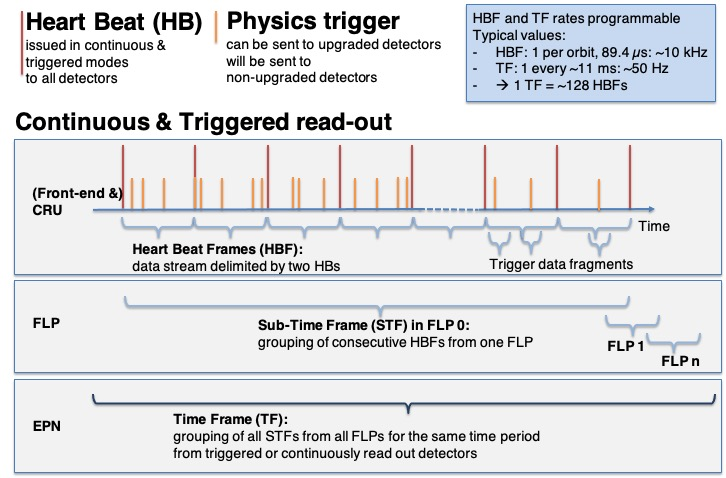
\includegraphics[width=1.\textwidth]{../fig/cru/tf_hbf_structure.jpg}
  \end{center}
  \caption{TF and HBF structure: additional info will be added here@}
  \label{fig_ro:tf_hbf_structure}
\end{figure*}

\begin{figure*}[hbtp]
  \begin{center}
    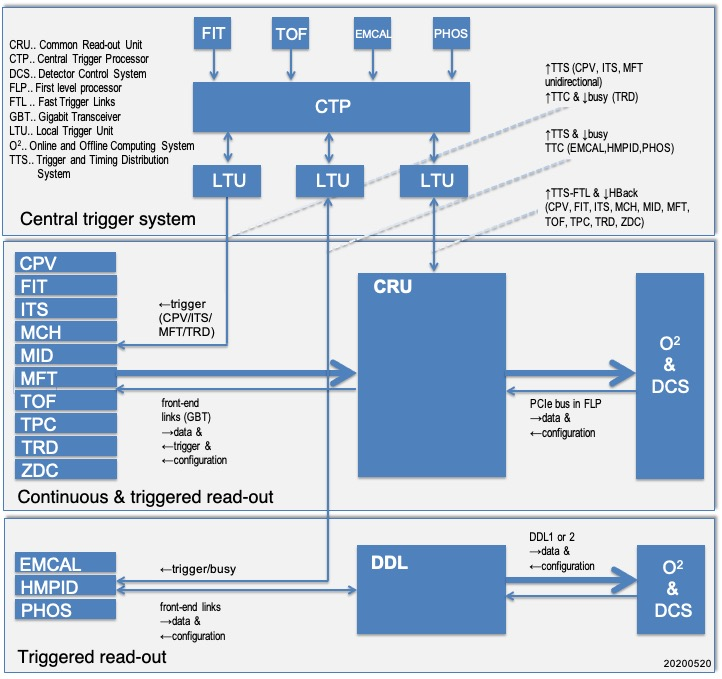
\includegraphics[width=1.\textwidth]{../fig/cru/ro_architecture.jpg}
  \end{center}
  \caption{ALICE read-out architecture: additional info will be added here@, add FLP and EPN farm}
  \label{fig_ro:ro_architecture}
\end{figure*}

\begin{figure*}[hbtp]
  \begin{center}
    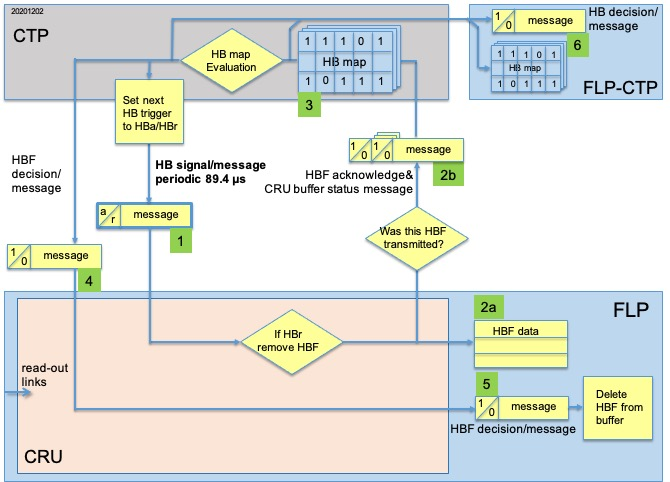
\includegraphics[width=1.\textwidth]{../fig/cru/control_signals.jpg}
  \end{center}
  \caption{ALICE Control signals: additional info will be added here@ or the figure will be removed}
  \label{fig_ro:control_signals}
\end{figure*}





\begin{itemize}
\item Radiation tolerance/load
\item continuous read-out, no filtering but compression (general description), TF and its related impact on reconstruction, CTP-CRU-FLP-EPN approach, implementation specification (beam, particle load, radiation load)
\item beam pipe
\item installation sequence, maintainability of ITS
\end{itemize}


\section{Chip developments (12 p.)}
\subsection{ALPIDE (Vito)}

\subsection{SAMPA (Marcelo, Alex)}



\section{Detector systems}
(aim for similar substructure for all detectors)

Some words on setup overview \dots

\begin{figure}
\centering
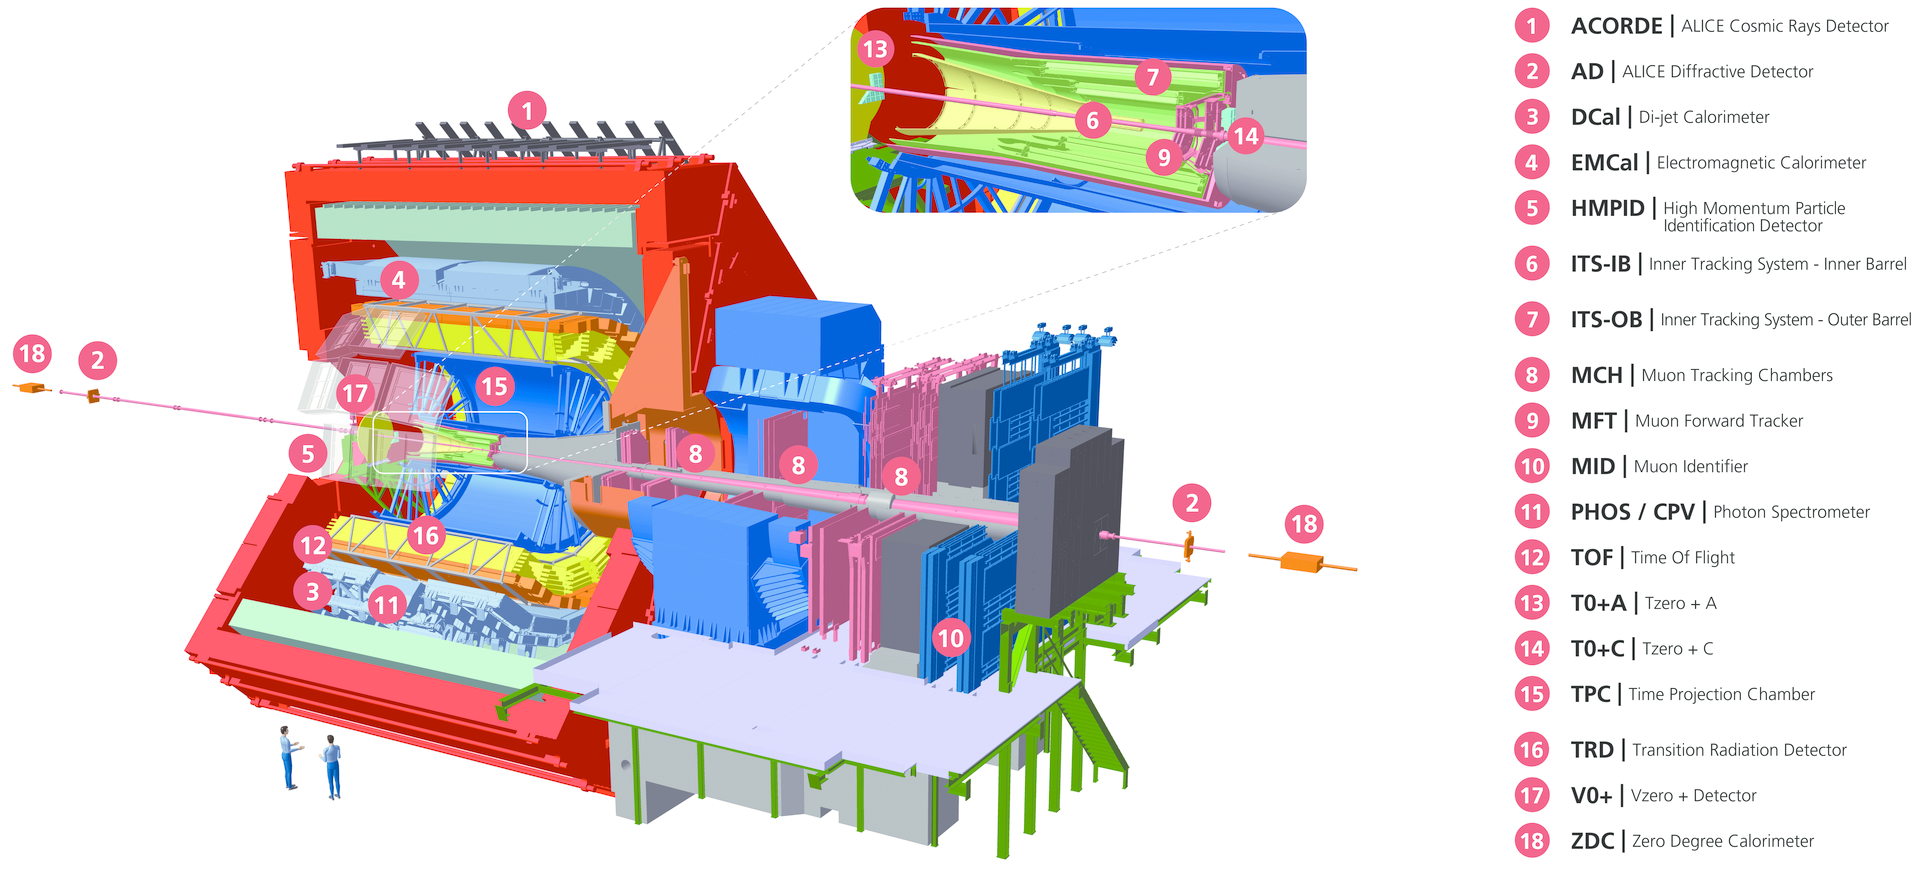
\includegraphics[width=.5\textwidth]{common/2017-May-11-ALICE_RUN3_labels_HD}
\caption{Overview Run 3}
\label{fig:alice_run3}
\end{figure}

\subsection{ITS (Vito; 10 p.)}

\subsection{MFT (Raphael 5 p.)}

\subsection{TPC (Harry; 10 p.)}



\subsection{Fast Interaction Trigger (FIT)}

\begin{figure}[htbp]
\begin{center}
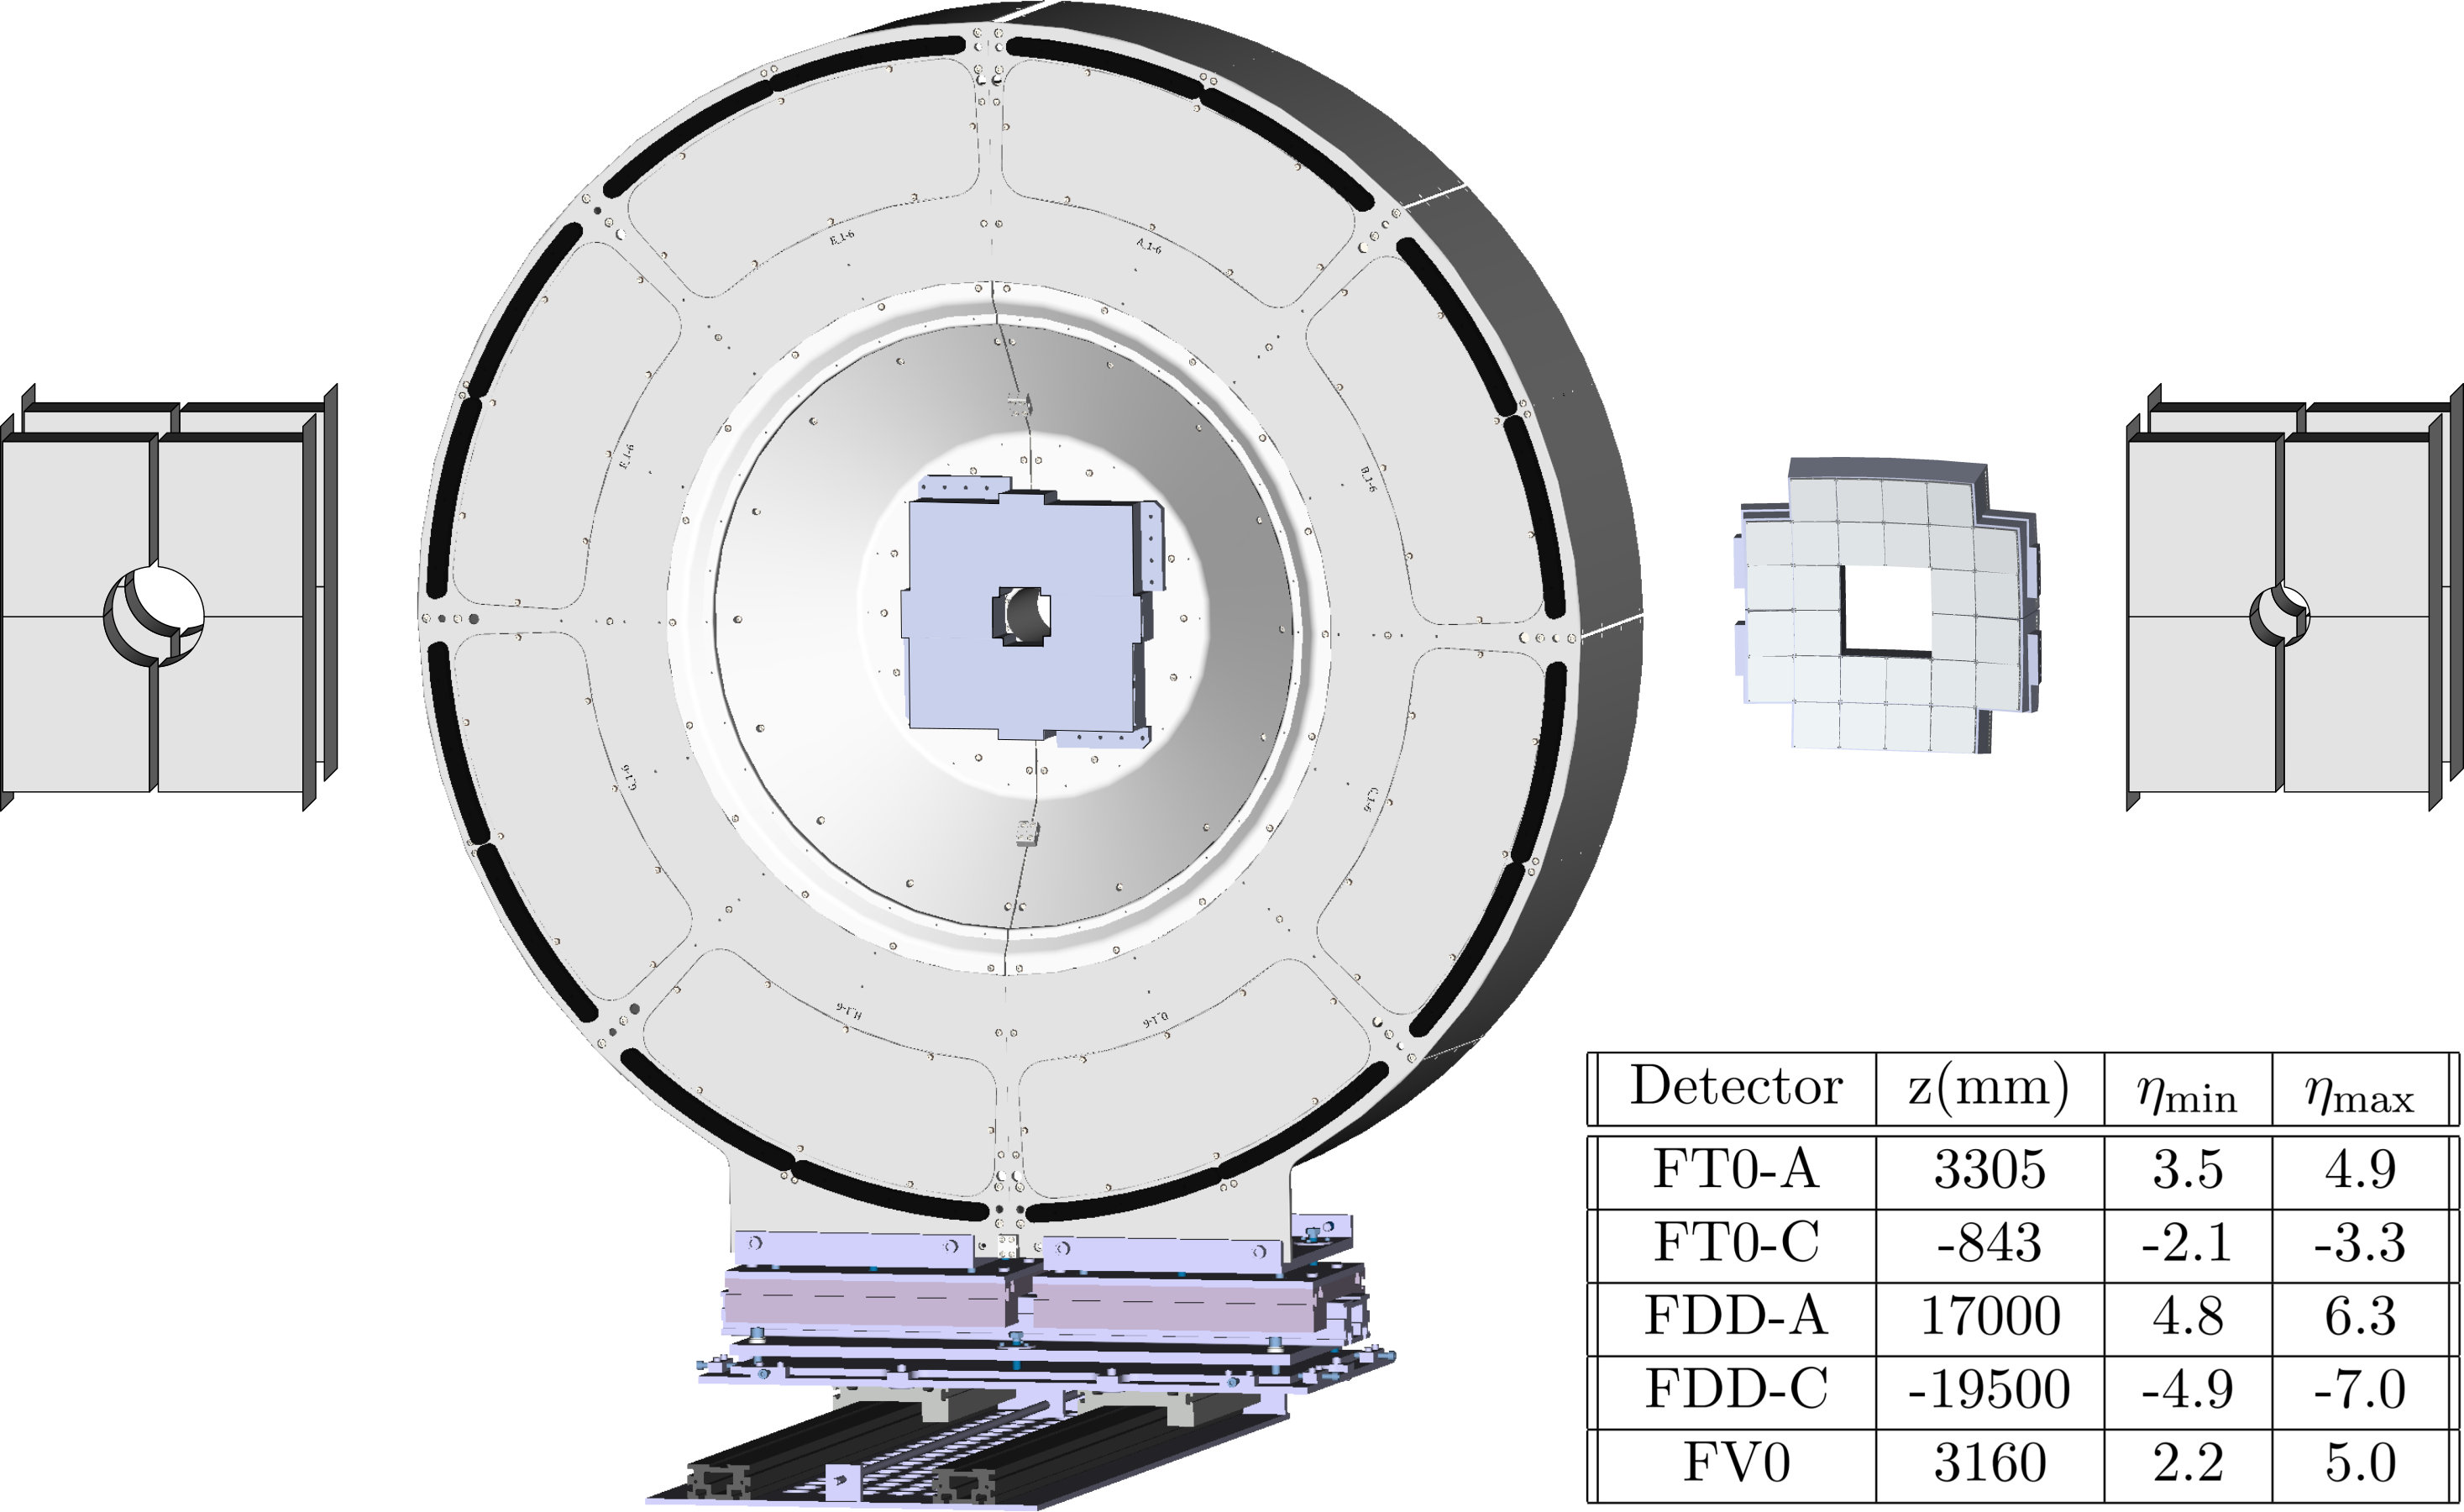
\includegraphics[width=0.8\linewidth]{fit/f40Fit3dCompleteTable.png}
\caption{View of FIT detectors illustrating the relative sizes of each component.  From left, FDD-A, FT0-A, FV0, FT0-C, FDD-C.  Note that FT0-A and FV0 have a common mechanical support. FT0-A is the small quadrangular structure in the centre of the large, circular FV0 support. Note that all are planar with the exception of FT0-C which has a concave shape centered on the IP.  The inset table lists the distance from the IP and the pseudorapidity coverage for each component.  }
\label{FITschematic}
\end{center}
\end{figure}

The Fast Interaction Trigger (FIT)\cite{Trzaska:2017reu} serves as an interaction trigger, online luminometer, initial indicator of the vertex position, and the forward multiplicity counter. In the offline mode it provides the precise collision time for the TOF-based particle identification, yields the centrality and interaction plane, and measures cross sections of diffractive processes. To deliver the required functionality, the active elements of FIT use three different detector technologies grouped into five arrays, as shown in fig.~\ref{FITschematic}. Their distance from the IP and their pseudorapidity coverage are displayed in the inset table in .~\ref{FITschematic}. The naming convention relates to the similar ALICE detectors used during Run 2. FT0 is the successor of T0~\cite{Bondila:2005}; FV0, of V0~\cite{V0performance:2014}; and FDD, of AD~\cite{broz:2020mb}. The main reason for the upgrade is the increased luminosity and interaction rate~\cite{Trzaska:2020zzl}, which can reach 1 MHz in proton$-$proton (pp) and 50 kHz in Pb$-$Pb collisions during LHC Runs 3 and 4. To cope with the increased interaction rate and to enable continuous readout, a new fast electronics and readout system~\cite{Finogeev:2020qkf} have been designed and implemented for all FIT subdetectors.

%In order to maintain the physics performance of the detectors replaced by FIT, FT0 is optimized to provide very good timing and a highly efficient fast multiplicity trigger, FV0 allows for the measurement of multiplicity as a function of pseudorapidity and azimuthal angle, and FDD's  coverage at small angles with respect to the beam gives access to measurements of diffractive processes. FT0 and FDD have arrays on either side of the nominal interaction point; FV0, due to severe space constraints, is only on the A side. 


 \subsubsection{FT0}
 
The FT0 consists of two
arrays, FT0-A and FT0-C, of  quartz Cherenkov radiators optically coupled to Photonis XP85002/FIT-Q microchannel
plate-based photomultipliers (MCP), which are factory customized versions of the Planacon XP85012. The modification is a new back-plane designed specifically for FT0 grouping the 64 anodes into 4 outputs. The 4 independent outputs deliver signals from 4 optically isolated 2\,cm thick  $2.65\times 2.65 \,\rm{cm}^2$  quartz radiators.  The signal path from each anode is the same length to improve the timing properties of the system.  This segmentation allows for providing the granularity for measurements of  multiplicity in central Pb$-$Pb collisions and has very good coverage of the solid angle subtended by the detector.  The intrinsic time resolution of each quadrant is  $\sigma_{\rm t} \approx 13\, {\rm ps}$ \cite{Melikyan:2020owp}. Accounting for signal deterioration along the 30 m long signal cables and processing by the 
front-end electronics, the achieved one-MIP time resolution of FT0 is about 25\,ps.  
The efficiency of the Minimum Bias trigger for pp collisions is  $\geq 98\%$ for the OR of the two sides and  $\geq 77\%$ for coincidences between FT0-A and FT0-C.
%\begin{figure}[htbp]
%\begin{center}
%\includegraphics{FT0C.jpg}
%\caption{Support structure for the FT0-C.}
%\label{FT0Cfig}
%\end{center}
%\end{figure}


FT0-A, located 3.3 m from the IP has 24 modules and thus 96 individual readout channels.
Due to the close proximity to the IP, the FT0-C support has a convex shape (as seen from the IP) positioning all 28 MCPs such that each of the 112 quartz radiators is 84 cm from the nominal IP.
 
\subsubsection{FV0}
FV0 is a large, segmented scintillator disk with a novel light collection scheme \cite{grabski2019new} assuring short pulses, single MIP time resolution of $\approx 200\, \rm{ps}$  , and a very uniform response across the entire detection surface. The active element of FV0 is a 4 cm thick EJ-204 plastic scintillator divided into 5 concentric rings of equal pseudorapidity coverage. The outer diameter of the largest ring is 144 cm and the inner diameter of the smallest is 8 cm. The 4 inner rings are subdivided into 8 sectors of 45 degrees each while the outermost ring, due to its large area, has 16 sectors. A grid of equal-length, clear Ashai fibres is attached to the back side (as viewed from the IP) of the scintillator as can be seen in fig.~\ref{FV0fig} At the other end, the fibres from each sector form a bundle and are optically coupled to Hamamatsu R5924-70 PMTs. This way, the 48 sectors of FV0 deliver 48 independent readout channels. This segmentation, combined with the information from the other forward detectors, is sufficient to yield the required centrality and event plane resolution. Together with FT0, FV0 provides the needed input to generate Minimum Bias and Multiplicity trigger at the LM (Level Minus one) level. Having the total latency below 425\,ns, this is the fastest trigger in ALICE. In addition, the FV0 monitors LHC background conditions and luminosity. 

\begin{figure}[htbp]
\begin{center}
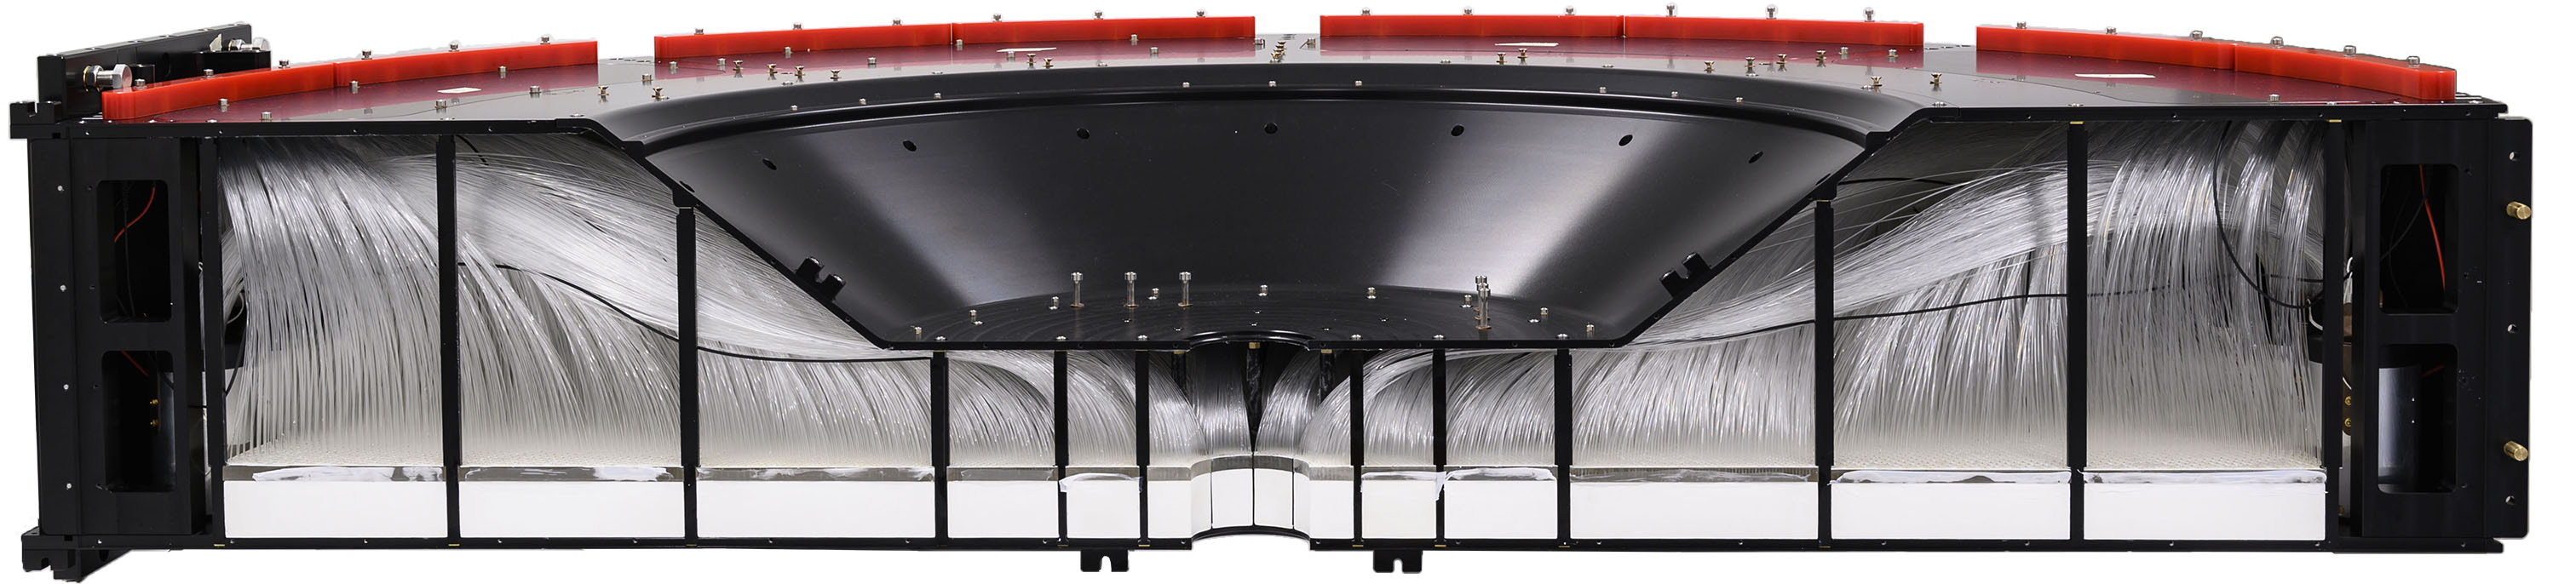
\includegraphics[width=0.9\linewidth]{fit/FV0_crossSection.jpg}
\caption{ Photograph of one half of the FV0. The optical fibers connect the scntillators to the PMTs on the rim of the support structure, the black structure seen here. The center wall has been removed to show the scintillator, surface matrix structure, and optical fibers.}
\label{FV0fig}
\end{center}
\end{figure}


\subsubsection{FDD}
The FDD \cite{Rojastorres} comprises  two nearly identical arrays, FDD-A and FDD-C, surrounding the beam pipe on opposite sides of the IP.  Each array consists of eight rectangular pads, $216 \times 181 \times 25\, \rm{mm}^3$ BC420 scintillator. The pads are assembled as  two overlapping layers of four sectors each. To make clearance for the beam pipe, a quadrant was removed from the innermost corner of each scintillator plate. The diameter of the removed quadrant on the FDD-A scintillators is 124 mm and 74 mm on the FDD-C as illustrated in fig.~\ref{FITschematic}. Each pad has two wavelengths shifting (WLS)
bars attached to the opposite sides of the scintillator. Clear optical fibres carry the light
from the WLS to H8409-70 PMTs. There are 8 independent FDD channels on each side of the IP.

Benefitting from the much improved ITS capability of heavy flavour tagging in the central barrel, the FDD contributes to the measurements of diffractive cross sections and studies of ultra-peripheral collisions. In pp collisions, the main physics objectives of the FDD are the studies of centrally produced exclusive states, measurements of cross sections for single and double diffraction, and inelastic processes at the new LHC centre of mass energy of 14 TeV. In Pb$-$Pb and p$-$Pb collisions, the FDD provides an independent measurement of centrality in an intermediate pseudorapidity range between the ITS and the ZDC and contributes to the selection of ultra-peripheral collisions. In the online mode, the FDD is used to monitor beam quality and to reject beam-gas events. 


\subsubsection{Electronics and readout scheme}

\begin{figure}[htbp]
\begin{center}
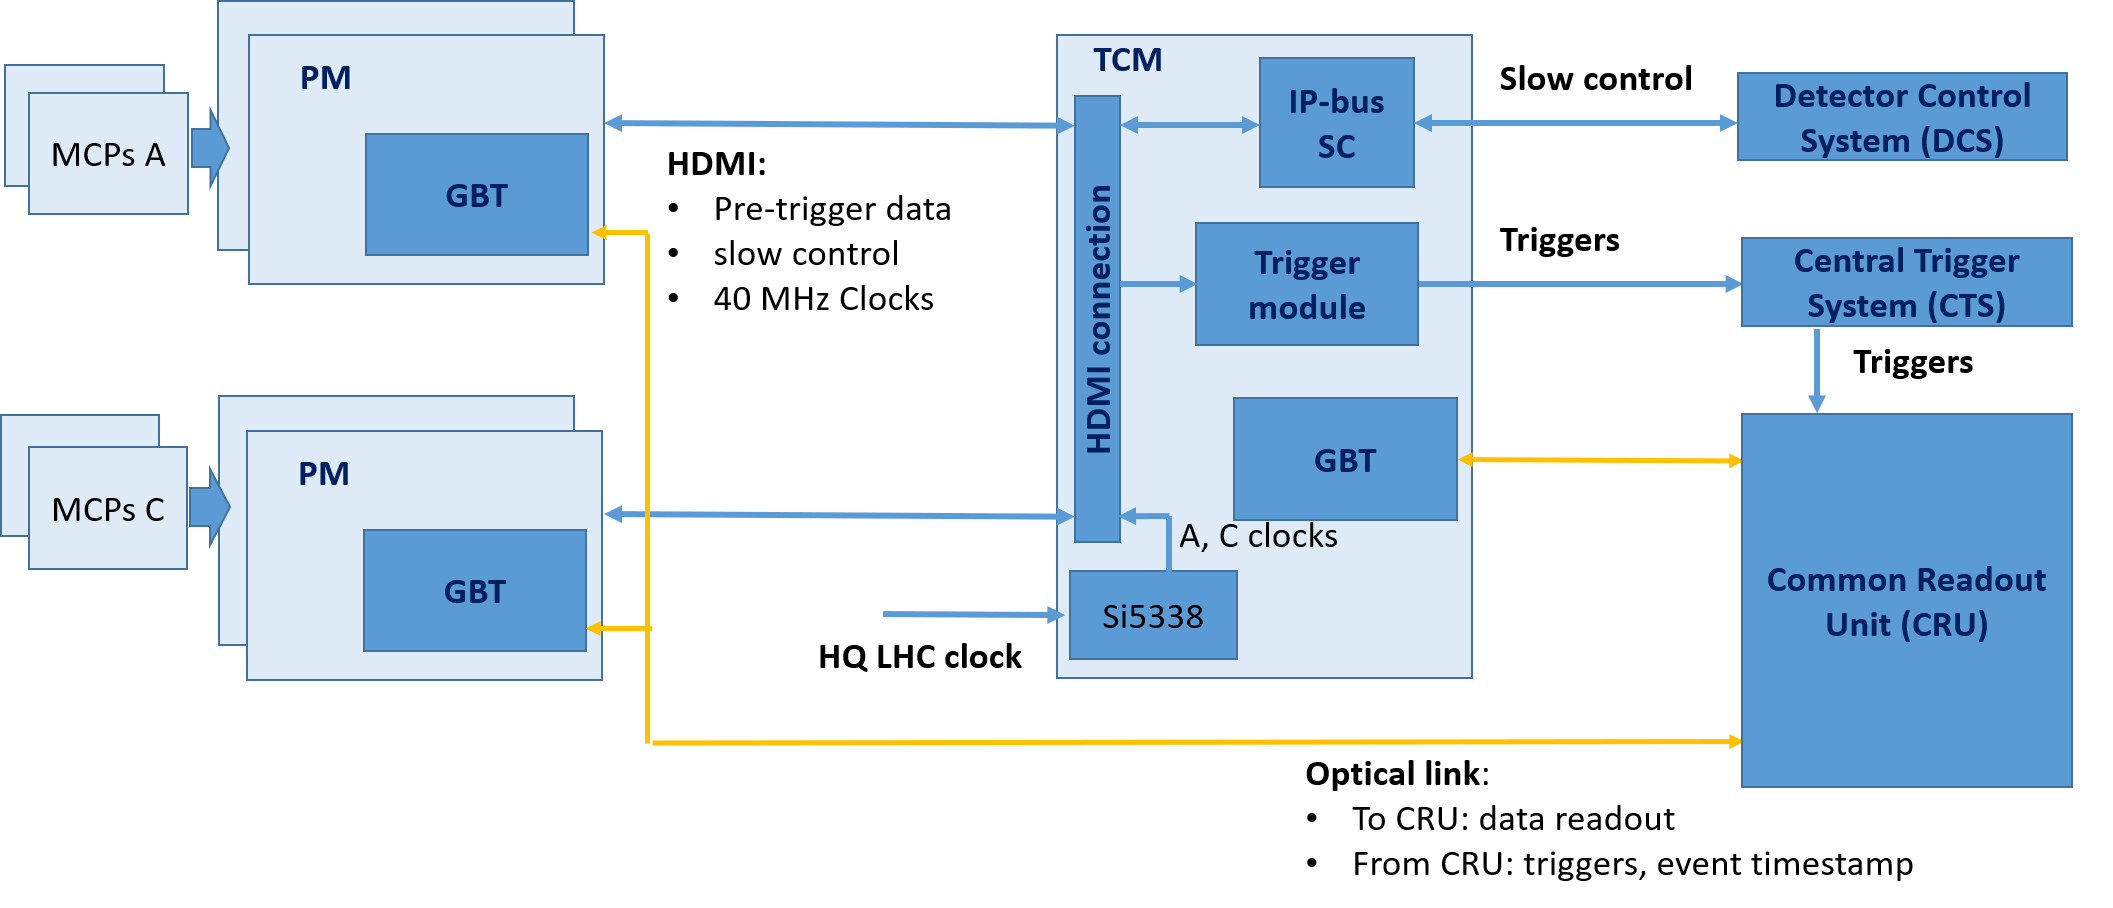
\includegraphics[width=0.9\linewidth]{fit/FIT_data_processing.png}
\caption{Schematic diagram of the FIT readout electronics. }
\label{default}
\end{center}
\end{figure}
All three subsystems of FIT use the same front-end and readout electronics based on just two custom-designed modules: a Processing Module (PM) and a Trigger and Clock Module (TCM). One PM provides 12 independent inputs. Each sub-detector has only one TCM while the number of PMs is determined by the number of channels. Each PM is connected to the dedicated TCM via an HDMI cable to transmit "pre-trigger" data, slow-control data and LHC clock distribution. The commands, configuration data, and status data are sent from the ALICE control system to the TCMs via a 1 Gb Ethernet optical link using an IPbus (UDP
based protocol) \cite{Finogeev:2020qkf}. The triggers and the measured event rates for the luminosity
measurements are transmitted from the TCMs via the same connection. The PMs are
configured from TCMs via an HDMI SPI connection. The PMs and TCMs are connected
to the ALICE DAQ with GBT links. FIT delivers the produced trigger signals to the Central Trigger System.
 
Laser pulses are used for time and amplitude calibration, as well as monitoring of ageing and radiation damage of the FIT detectors.


\subsection{Muon System (8 p.)}
\subsubsection{Muon Tracking (Herve; 5p.)}
\subsubsection{Muon Identifier (Pascal; 3p.)}

The Muon Identifier (MID) is the present designation of the Muon Trigger system~\cite{Aamodt:2008zz} which was operational in ALICE during LHC run~1 and run~2. 

The detector is composed of 72 single gap Resistive Plate Chamber (RPC) detectors, organized in two stations of two planes each, located at 16~m and 17~m from 
the interaction point. The planes in the same station are 17~cm apart. The total detection area is about 150~m$^{\rm 2}$. An overview picture of one half-plane of the MID, in open position, taken during the FEERIC card 
installation (see next section) in 2019, is shown in Fig.~\ref{midhalfplaneopen}.

The RPC signals are collected by means of a total of 20992 readout strips, each of them equipped with Front-End (FE) electronics. The output signals from the FE electronics, in LVDS electrical standard of 25~ns width, 
are propagated via multi-wire copper cables to the readout electronics (also in charge of the muon trigger decision during run~1 and run~2). 

\begin{figure}
\centering 
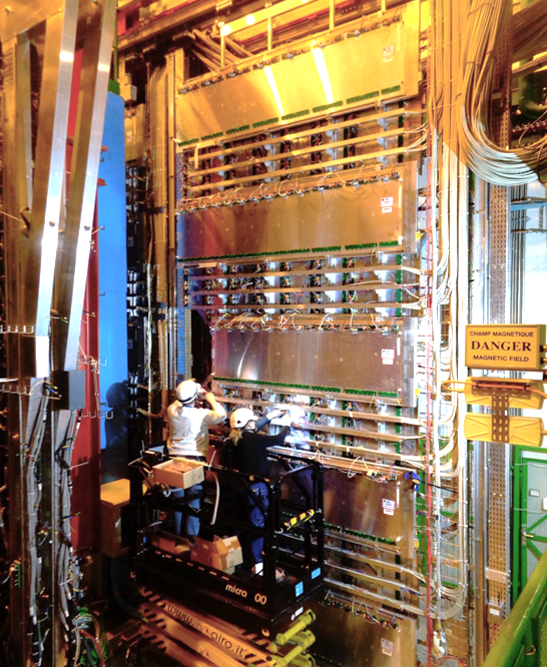
\includegraphics[width=.4\textwidth]{mid/midhalfplaneopen}
\caption{Overview of one MID half-plane in open position}
\label{midhalfplaneopen}
\end{figure}

The FE electronics cards, located on the RPC detectors, have been replaced during the LS2. The main motivation is to reduce the ageing of the RPCs during future data taking periods. 
The FE ASIC of the past FE electronics, called ADULT~\cite{mid:ADULT}, has been upgraded to a new one, called FEERIC~\cite{mid:FEERICref1,mid:FEERICref2}.
Unlike ADULT, FEERIC performs amplification of the RPC analog signals. Thanks to this upgrade, the ALICE RPCs will be operated in avalanche 
mode after the LS2 with a significant reduction of the charge produced in the gas gap as compared to past conditions, hence limiting ageing effects.

The readout electronics (more than 250 complex electronics cards) have been also completely replaced for sustaining the large data flow going with the future high collision rate. 
The new system is designed for continuous readout so there is no more need for hardwired muon trigger signals, the event selection being done at the online processing level. 

All RPC detectors were still operational at the end of run~2. However few of them were drawing a relatively large current after having accumulated up to 20~mC/cm$^{\rm 2}$.
It was therefore decided to replace those RPCs by completely new produced ones. For the longer term, a crucial R\&D on new environment-friendly 
gas mixtures~\cite{mid:RPCgasmix} for RPCs, based on tetrafluoropropene which is characterized by a very low Global Warning Potential (GWP), has been launched.


\paragraph{FEERIC electronics\\}
 
The FEERIC 8-channel ASIC is designed in the AMS 0.35~$\mu{\rm m}$ CMOS technology. It is mostly composed (see Fig.~\ref{midFEERIC}, top scheme) of a transimpedance amplifier, a zero-crossing discriminator and a one-shot 
which prevents retriggering during 100~ns. The operating threshold is typically 70~mV corresponding roughly to 130~pC at readout strip level. Details of the performance of the FEERIC electronics 
is given in~\cite{mid:FEERIC-PRR}. Figure~\ref{midFEERIC}, bottom, shows a picture of a FEERIC card. 2720 cards (spare included) have been produced in the second half of 2017.
The installation of the FEERIC cards on the RPCs in ALICE cavern has been completed in July 2019. 

In parallel, a new wireless threshold distribution for the FEERIC cards has been developed. 
A total of two masters (one per side of the cavern) and 24 nodes close from the RPCs (see Fig.~\ref{midTHRdistri}, picture on the right), installed in ALICE cavern in 2019, allows to remotely control the threshold of each of the 2384 installed 
FEERIC cards. The masters are controlled via ethernet and communicate via the high level ZIGBEE wireless protocol with the nodes which are themselves I2C chained to the FEERIC cards on the RPCs (see Fig.~\ref{midTHRdistri}, 
scheme on the left). Master and node share the same hardware and firmware. Card acts as master or node depending on the configuration stored in EEPROM which also keep memory of the last requested threshold values, restored
at power on.  

During run-2, one of the 72 ALICE RPCs was equipped with FEERIC electronics and the wireless distribution, showing satisfactory performance and stability. The charge released in the gas (25-30~pC per hit) is four times less 
than the one of RPCs with ADULT.

\begin{figure}
\centering 
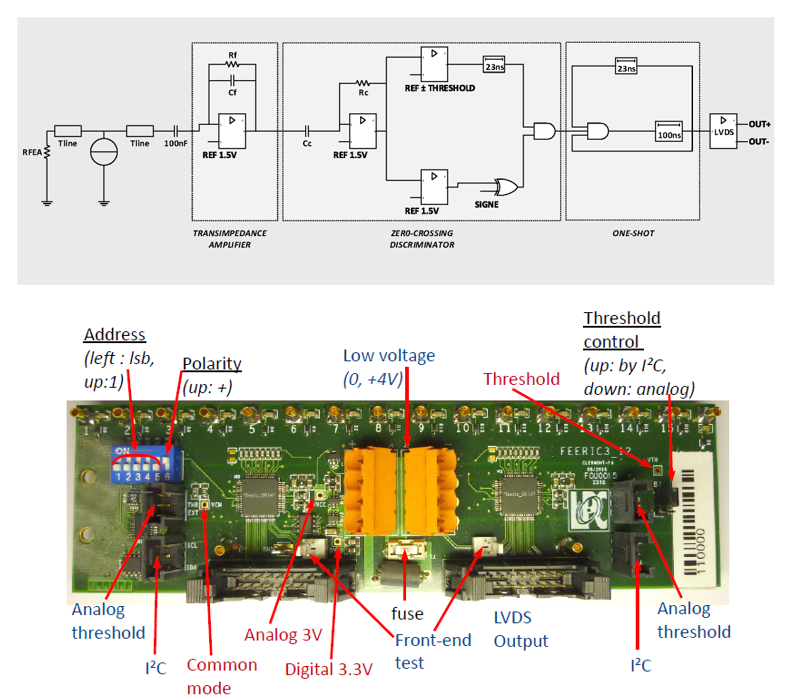
\includegraphics[width=.5\textwidth]{mid/midFEERIC}
\caption{FEERIC ASIC architecture (top) and FEERIC card picture (bottom)}
\label{midFEERIC}
\end{figure}

\begin{figure}
\centering 
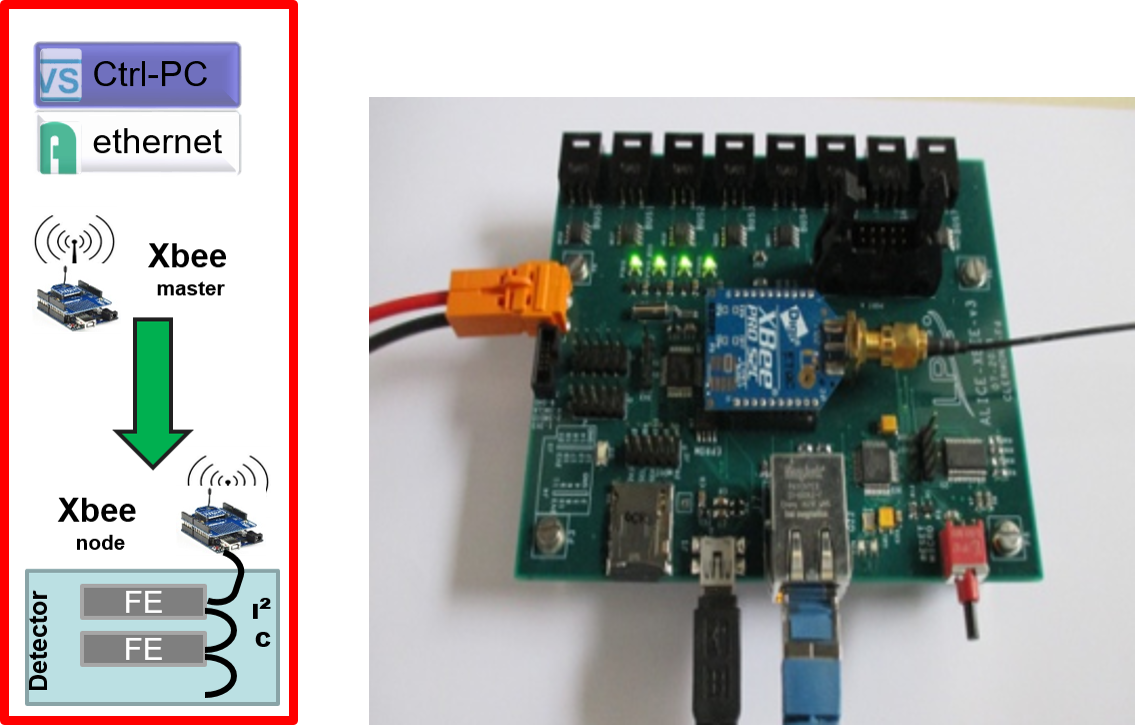
\includegraphics[width=.5\textwidth]{mid/midTHRdistri}
\caption{Wireless threshold distribution scheme (left) and master or node electronics card (right)}
\label{midTHRdistri}
\end{figure}




\paragraph{Readout electronics\\}

The LVDS (binary) signals from the FE electronics, so called strip-patterns of length 16 bits, are received by the Local cards. 
Each Local receives strip-patterns from the four detector planes, each of them from the two orthogonal coordinates (from horizontal and vertical readout strips on both sides 
of the same RPC). The whole project consists in 234 Local cards, housed in 16 VME-9U crates used as mechanical support and for power supply. 
The Regional card in the crate communicates with a maximum of 16 Local cards via the e-links of the J2 bus. Each Regional card is interfaced to a Common Readout Unit (CRU) by means of two GBT links at 3,2~Gbit/s. 

The project has a total of two CRUs only, housed in one single First Level Processor (FLP) tower PC. The MID readout architecture is shown in the left panel of Fig.~\ref{midRO} while a picture of the three types of readout cards 
is shown on the right. Simulations of the expected bandwidth for Pb--Pb collisions at 50~kHz, based on run~2 real data, indicate that 
this design includes a safety factor of more than one order of magnitude. 

Data corresponding to so-called self-triggered physics events~\cite{mid:ROweb,mid:DataNote} are transmitted from the Local and Regional to the CRU. There is potentially a new event stored 
in the Local and Regional FIFOs each 25~ns. Information is stored in these FIFOs only in case of a non-empty event which, in standard configuration,
corresponds to at least two coordinates in the same detector plane with non-zero bit-patterns. 
It is important to note that it takes five clock cycles (at 40~MHz) per self-triggered event for the transfer of the Regional FIFO and 9-21 clock cycles for the transfer of the Local FIFO, depending on the
number of non-empty planes in this last case. As a first consequence, the data from Local and Regional corresponding to the same bunch crossing (BC) arrive asynchronously in the CRU. As a second consequence, the
Local and Regional FIFOs would go to saturation in case of filling at the full clock frequency, corresponding for example to a very high level of noise at the FE level: a busy bit would be set in such case.

The CRU user logic (UL), first stage of data processing in the CRU, is essentially performing zero-suppression and raw data header construction using the central trigger (CTP) orbit information. 
The UL output is transmitted by words of 256 bits to the FLP. At this level, the data coming from the different GBT links are assembled in C++ structures and synchronized to provide the information 
corresponding to a given interaction. The readout electronics always operates in continuous readout mode. However the system can also handle triggered mode, selecting those events in coincidence with a trigger from the CTP, either 
in the CRU or the FLP.

The Local and Regional respond (see~\cite{mid:ROweb}) also to all types of central triggers issued by the CTP and received via the GBT down-link. 




\begin{figure}
\centering 
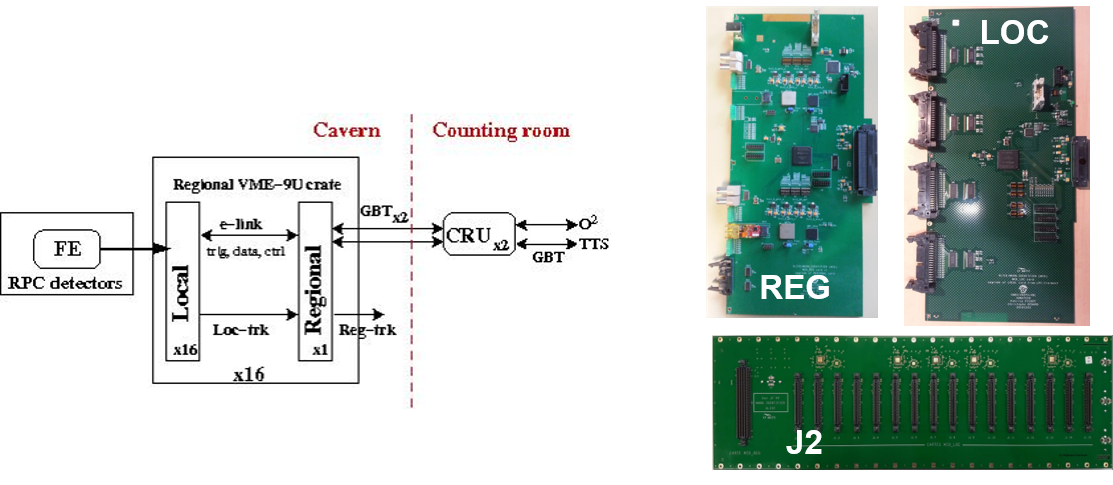
\includegraphics[width=1.\textwidth]{mid/midRO}
\caption{MID readout architecture (left) and readout cards (right picture) with Local (top right), Regional (top left) and J2 bus (bottom ) between Local and Regional}
\label{midRO}
\end{figure}






\subsection{TRD (Johanna; 3 p.)}

\subsection{TOF (Pietro; 3 p.)}

\subsection{HMPID (Giacinto; 2 p.)}

\subsection{EMCal (Constantin; 2 p.)}

\subsection{PHOS (Yuri; 2 p.)}

\subsection{ZDC}

The aim of the ZDC upgrade is to cope with the high collision rate foreseen after LHC LS2 upgrade. The calorimeters sustained well irradiation during RUN1/2 operation, therefore don't need to be replaced. The two items that required attention were the consolidation of the infrastructure and the upgrade of the readout system.

The first item required two main actions. Firstly it involved the upgrade of the control electronics of the movable platform sthat bring the ZDC calorimeters in a garage position where it is shielded by potential beam losses during beam injection or adjustment operations and allow to align them with the neutron (proton) spot during data taking. A second action involved the installation of additional power supplies for the voltage dividers of the ZDC photomutipliers to stabilize the gain in the high event rate conditions that are foreseen. 

The main upgrade activity concerned a new readout system based on faster electronics. In fact the RUN1/2 readout electronics was based on VME QDCs with a conversion time of $\sim\SI{10}{\micro\second}$ that cannot cope with a $\SIrange[range-units=single,range-phrase=\div]{50}{100}{\kilo\hertz}$ event rate without dead time. Moreover, in order to fully exploit the ALICE physics potential in ultra-peripheral heavy ion collision, the ZDC aims at taking data in continuous (autotrigger) readout mode. This operating condition is particularly challenging since the ZDC has acceptance not only to nucleon emission from hadronic interactions but also to the ones resulting from electromagnetic dissociation \cite{Pshenichnov2001,Pshenichnov2011,ALICE:2012aa} that have a much higher cross section for Pb-Pb collisions at LHC energies and consequently the ZDC will be exposed to $\sim\SI{5}{\mega\hertz}$ total event rate.

Thanks to the low number of channels to be instrumented, the solution is based on commercial digitizers, in particular ALICE will use FMC digitizers that allow a continuous sampling of the signal waveform followed by a real time analysis on a FPGA. 
Thanks to the adequate bandwidth available through the FMC connection from the digitizer to the FPGA the full waveform can be analyzed. Fast trigger and reconstruction algorithms are executed on the FPGA and the interesting portions of waveform are transferred to the acquisition and reconstruction system through optical GBT links.

To preserve the time and charge resolution 
%of the present system
and to match the bandwidth of the ZDC signals, the digitizers should have about $\SI{12}{\bit}$ resolution (with an ENOB of $\sim\SI{10}{\bit}$) with a sampling frequency of
% $\SIrange[range-units=single,range-phrase=\div]{0.5}{1}{\giga\sps}$
$\SIrange[range-units=single,range-phrase=\div]{0.5}{1}{\giga\hertz}$. Since the PM signal is unipolar the digitizer has to be DC coupled (and this reduces the number of useful models available on the marked). After evaluating a few modules it was chosen the ADC3112 FMC \cite{IOXOSADC3112} mounting digitizer ADS5409 \cite{TIADS5409}. The FMC is hosted on the carrier IFC\_1211 \cite{IOXOSIFC1211} with a Kintex UltraScale XCKU40 FPGA. The ADC3112 on-board oscillator is locked to the LHC revolution frequency recovered from GBT link and dispatched through the FMC connector. The ADC will acquire 12 samples per bunch crossing, therefore it will run at
% $\sim\SI{960}{\mega\sps}$
$\sim\SI{960}{\mega\hertz}$. In order to reduce the data size the low pass filtering with digital downsampling is enabled on the ADC. This has the benefit of improving the measurement accuracy by averaging over the even and odd samples without the need to correct for the slightly different gain and offset that is present on this type of ADC. The data throughput to the FPGA will therefore be reduced to $\sim\SI{480}{\mega\sps}$ simplifying the firmware design.

A critical aspect of the ZDC operation in RUN3 is triggering at high rate in \PbPb with bunch spacing reduced to $\si{50}$ or $\SI{25}{\nano\second}$ since the PM signal will be comparable or longer than the bunch spacing. This is complicated by the large signal dynamics (from a one to $\sim60$ neutrons in the acceptance of the neutron calorimeters). In order to identify the presence of a signal a differential trigger algorithm has been developed. Samples at different times are compared (sample $y_{\textrm{i}}$ with sample $y_{\textrm{i+shift}}$ where $\textrm{shift}$ is a tunable parameter from 3 to 5 samples). If three successive differences are above threshold $th$, i.e. $\left(y_{\textrm{i}}-y_{\textrm{i+shift}}\right)>th\,\&\,\left(y_{\textrm{i+1}}-y_{\textrm{i+shift+1}}\right)>th\,\&\,\left(y_{\textrm{i+2}}-y_{\textrm{i+shift+2}}\right)>th$ 
the trigger condition is satisfied, effectively rejecting fake triggers due to electronic noise, and the bunch is flagged for acquisition. This autotrigger condition drives the acquisition in continuous readout mode while in triggered mode the readout system acquires data regardless of the autotrigger flag. The same flags are used also to measure the interaction rate that is used to estimate the instantaneous luminosity.

The measurements of signal arrival time and amplitude need to take into account the baseline (pedestal) oscillations and the possible presence of a signal in an earlier bunch crossing (pile-up).

Two methods for pedestal evaluation have been implemented. Given the bunch structure of LHC that alternates “trains” of colliding bunches to “gaps” where no collisions can occur, it is possible to measure the pedestal considering portions of the digitized data where no collision can occur. These are identified by a bit map uploaded on the frontend at each fill. Using this information the pedestal average for each LHC orbit is computed and then transmitted on GBT. This allows taking into account a possible low frequency drift of the baseline and obtaining an accurate reference. A second method allows to effectively subtract pedestal in presence of noise at higher frequencies. For each trigger (or autotrigger), in addition to the bunch where the signal peaks ($BC_0$), the 12 samples of the preceding bunch crossing ($BC_{-1}$) will be transferred in order to evaluate and subtract the pedestal, in case of significant discrepancy with the orbit average computed with the first method.

For what concerns the pile-up from a signal in an earlier bunch crossing, in autotrigger mode all ZDC signals are transmitted and reconstructed, allowing to identify and correct for pile-up. On the other hand, in triggered mode, the firmware ensures that the information on the signal inducing pile-up is not lost due to trigger selectivity. Consequently for each triggered bunch crossing up to four bunch crossing will be transferred: the triggered and the preceding one (pedestal evaluation) and additionally $BC_{-2}$ and $BC_{-3}$ in case a pile-up signal is detected.

During \PbPb data taking in 2018 a prototype of the ZDC system was tested in parallel to the ALICE data acquisition by using a custom system based on a Xilinx evaluation board readout with Labview. An example of the achieved performances is shown in Fig. \ref{fig:zdc-signals}. The resolution on $\SI{2.76}{\tera\electronvolt}$ single neutron emission detected by ZNC is $\sim17\%$, with an improvement w.r.t. the $\sim20\%$ of present electronics, and the time resolution w.r.t. the ALICE L0 trigger is $\sim\SI{0.35}{\nano\second}$ that is comparable with the performance of the present system.

\begin{figure}
    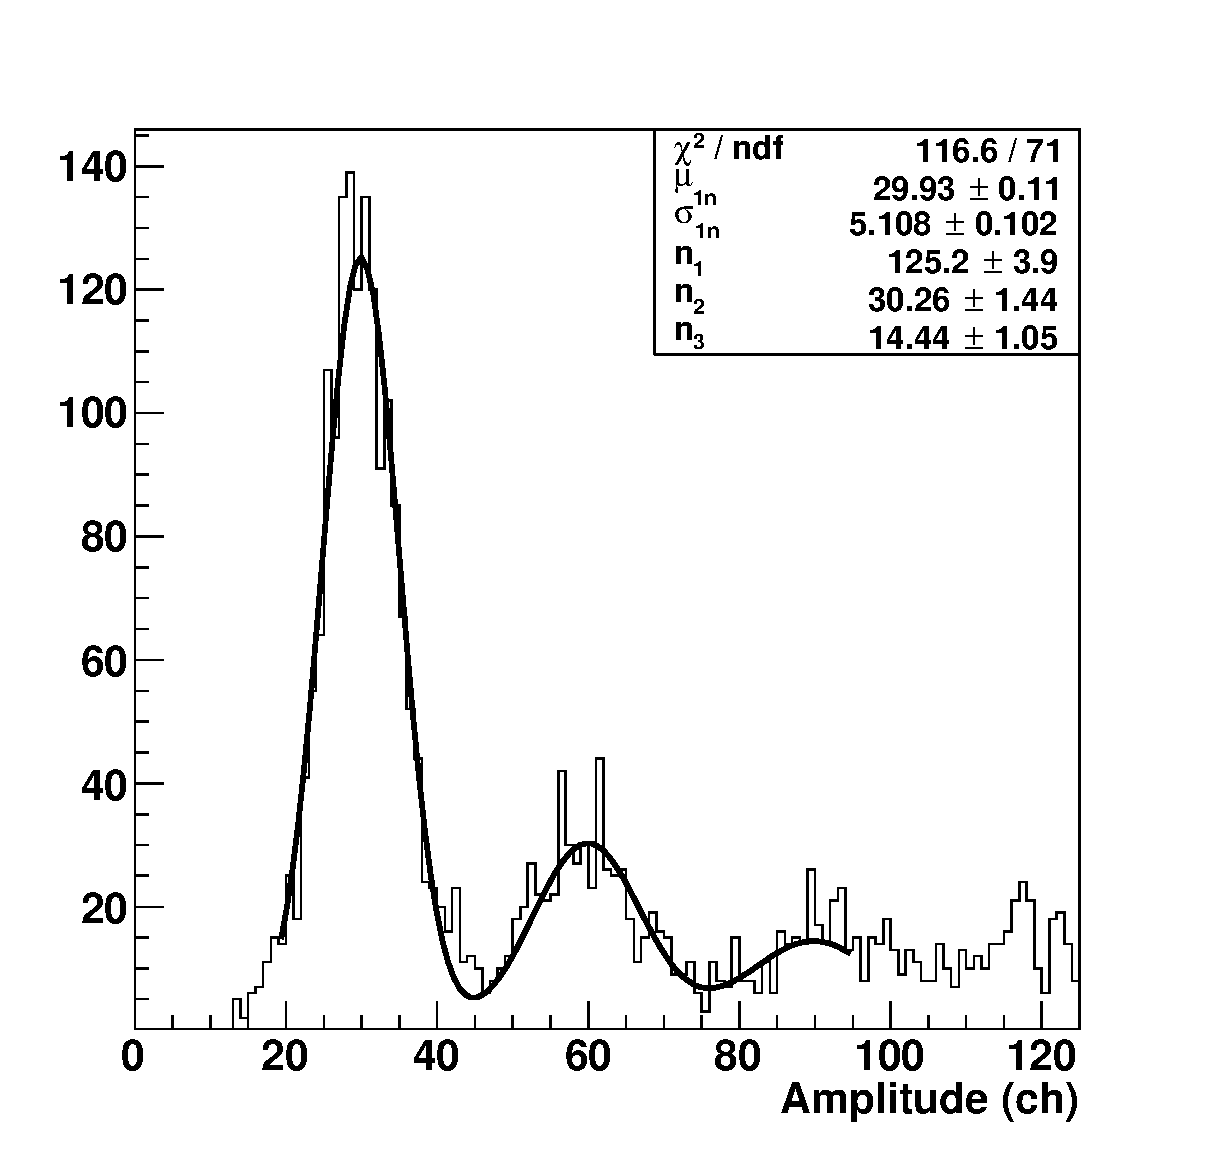
\includegraphics[viewport=0bp 0bp 569.4bp 736.111bp,clip,width=0.5\columnwidth]{zdc/fill_7457_dcmtnon_1n_resolution}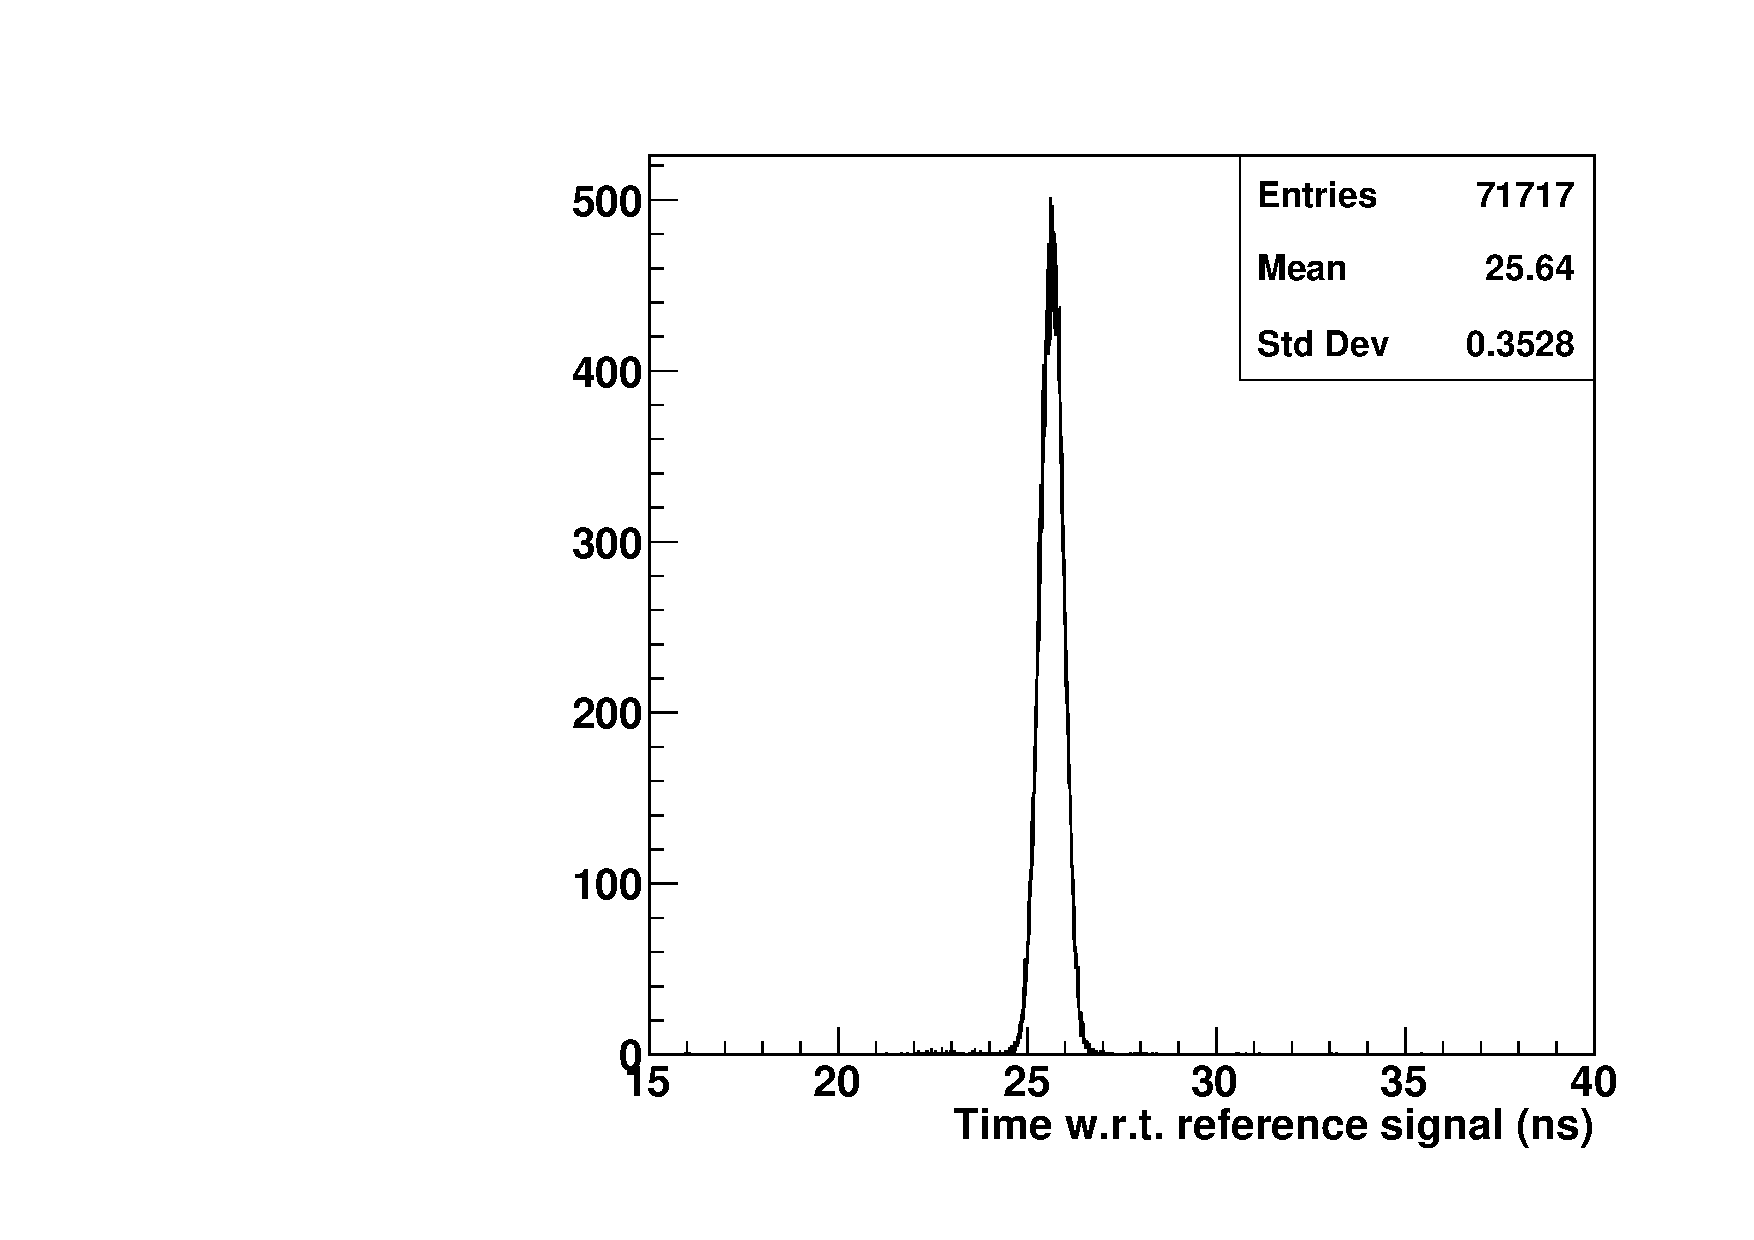
\includegraphics[viewport=0bp 0bp 569.4bp 736.111bp,clip,width=0.5\columnwidth]{zdc/run296549-part0-dcmtnon-d20181120-h1230_znctc_time}

    \caption{\label{fig:zdc-signals}On the left plot: the lower part of the triggered spectrum of ZNC common photomultiplier in Pb-Pb collisions where the emission of a single $\SI{2.76}{\tera\electronvolt}$ neutron  and multiples are visible. The autotrigger algoritm effectively rejects pedestal events. On the right plot: the arrival time of ZNC common photomultiplier
    signals w.r.t. the reference ALICE L0 trigger signal.}
\end{figure}



\section{Mechanics and integration (Werner, Corrado; 5 p.)}
Beampipe, support structures, detector alignment, installation and maintenance


\section{Read-out and data processing (20p.)}
%\subsection{O2 Overview: reconstruction workflow (PDP) (Andreas; 5 p.)}
\subsection{${\rm O}^2$ and Data Processing Overview}
In this section we give an overview of data processing from the detector read-out to the creation of analysis object data (see Fig. \ref{fig:02dp})
and then
focus on the processing steps that are synchronous with data taking.
The continuous read-out of the large majority of the detectors, is one of the most important changes with respect to Run1/2.
At the projected peak Pb--Pb interaction rate of 50~kHz the data throughput from the 
detectors is expected to be 3.75~TB/s, approximately a factor of 50 higher than during Run 2.
In order to minimize the costs and compute time of the offline system for data 
processing and storage, the ALICE Computing Model for Runs 3 and 4 is designed 
for a maximum reduction of the data volume synchronous with the data taking and without rejecting events. 
This task is achieved in two processing steps on the ALICE online/offline facility (${\rm O}^2$) located at Point2.
It consists of two types of compute nodes, the First Level Processors (FLP) located in the 
experiment access shaft (CR1) and the Event Processing Nodes (EPN) at CR0. In addition to the compute 
nodes it provides networking, data storage as well as interfaces with the Grid and the permanent data 
store at the Tier
0. For more technical details on these clusters, see sections \ref{sec:flp} and \ref{sec: epn}.

Data produced by the detectors are transferred to the common read-out units (CRU) in a continuous or
physics triggered read-out mode. The triggered data will be tagged with the LHC clock information while 
the continuous streams of data samples are split into so called heartbeat frames (HBF) tagged with the 
corresponding HB ID. Nominally, the time between two HBs is $89.4 \; \mu s$ (one LHC orbit period).
The data are compressed and multiplexed
in the CRUs and transferred to the memory of the FLPs.
The 272 FLPs perform a 
first level of data compression to 635~GB/s by zero suppression and clustering as well as calibration 
tasks based on local information from the part of the detector they serve, for example base-line 
correction.
Moreover, HBFs are accumulated into sub time frames (STF) of about 11-22~ms length (128-256 LHC orbits) 
containing $\approx 550-1100$ collisions. A dedicated FLP collects and processes data from the Detector 
Control System (DCS).
The STFs are then dispatched to the Event Processing Nodes (EPN). 

\begin{figure*}[hbtp]
  \begin{center}
    \vspace*{10cm}
  %\includegraphics[width=.5\textwidth]{<det>/<filename>}
 \end{center}
 \caption{O2 Data Processing Overview}
 \label{fig:o2dp}
 \end{figure*}

\subsubsection{Synchronous Reconstruction}

STFs related to the same time period and from all FLPs are received by the same EPN and aggregated into 
a complete time frame (TF).
The EPN farm consists of 250 servers hosting each 8 GPUs and 
64 CPU cores. The capacity has been dimensioned such that it can achieve
a first pass online synchronous reconstruction, extraction of calibration 
objects for subsequent asynchronous reconstruction passes and data reduction. 
Data is aggregated into so called compressed time frames (CTF) replacing the original raw data and 
written to a 
60~PB disk buffer at an output rate of 90~GB/s. Calibration data is aggregated and stored in the 
Calibration and Constants Data Base (CCDB). 

Two third of the CTFs are transferred to T0 and one third to T1 for archiving. 
After data taking and full detector calibration, at least two asynchronous 
reconstruction passes on T0 and T1 centers as well as on the EPN farm are 
performed. The output of these reconstruction passes is stored as Analysis 
Object Data (AOD), the input for physics analysis. For specific physics signals, a further data size 
reduction and speed-up of the corresponding analyses is achieved by filtering out events of interest and writing out only the minimum event information needed.
The processing of pp data will follow the same chain with the addition of the selection of interesting 
events during an asynchronous reconstruction pass with reduction of the CTFs by keeping only the 
clusters associated to these events. Reconstruction passes are followed by Monte Carlo production cycles taking into account the time dependent detector conditions.

Besides the compute infrastructure a common software framework has
been developed in collaboration with GSI (FAIR) within which all 
online and offline components are developed and operate. It 
consists of three main components. 
The {\it Transport Layer} is implemented using the FairMQ message 
passing toolkit. It enables efficient parallelism by providing 
abstraction of network and inter process communication as well as 
by supporting shared memory backed message passing. The {\it O2 Data 
Model} is message passing aware and provides support for various 
backends such as a performance optimized simplifies 0-copy format, ROOT based serialisation and Apache Arrow for analysis and and 
integration with external tools. Finally, the {\it Data Processing
Layer} (DPL) abstracts computation as a set of data processors 
organized in a logical dataflow explaining of data is transformed.

\begin{figure*}[hbtp]
  \begin{center}
    \vspace*{10cm}
  %\includegraphics[width=.5\textwidth]{<det>/<filename>}
 \end{center}
 \caption{Synchronous Reconstruction Workflow}
 \label{fig:rwf}
 \end{figure*}
\subsubsection{Synchronous Reconstruction}
A schematic representation of the synchronous reconstruction workflow is shown in Fig. \ref{fig:rwf}.
The main objective of synchronous processing is to reduce the data rate from the TPC which is with 90\%
the dominant contributor. This is achieved by performing clustering and full track reconstruction in the
TPC. Hits not attached to physical tracks are removed from the data. Moreover, cluster space point 
coordinates are stored as relative coordinates, thus reducing the entropy and allowing for very efficient entropy
encoding of the data.
In addition, detector calibration information is extracted replacing the additional 
calibration passes in front of the production reconstruction passes needed in Run1/2. TPC space charge 
distortion calibration uses the information of fully reconstructed barrel tracks including ITS, TOF and
TRD information. However, only a small fraction of all tracks are need to be reconstructed to gain 
sufficient statistics. Hence TPC reconstruction is the most compute demanding step. To be able to 
reconstruct Pb-Pb collision at a rate of 50 kHz in a cost 
effective way it is performed on Graphic Processing Units (GPU). They provide a significant speed-up 
with respect to CPUs (at least a factor of 50) without compromising the physics performance.

\subsubsection*{GPU Processing and Data Rejection}
TPC reconstruction starts with the cluster finding. It is followed by tracking comprising the track 
finding, track merging and fitting steps. These require a first order (average) space charge distortion
correction (see below). Two options for TPC data rejection are supported by the software. In the first 
option (A) clusters of identified background clusters (for example from noisy pads or charge clouds 
related to low momentum protons) and clusters associated to background tracks, such as very low momentum tracks, loopers and 
tracks with large inclination angle, are rejected.  For the second option (B) only clusters attached or
in the proximity of identified signal tracks are kept.
The estimated rejection fractions for options A and B are $12.5-39.1\%$ and $37-53\%$, respectively. 
While option B yields lower data size it is more risky in case of calibration problems. Optimal 
performance of option A requires identification of hits from particles with momentum below 10~GeV/$c$, 
which is still under development.

Further data size reduction is achieved by converting the cluster properties from the single-precision 
floating point format used in reconstruction to an integer format with exactly as many bits as needed 
for the intrinsic TPC resolution. For entropy reduction, coordinates of clusters that are not assigned 
to tracks are stored as differences to the previous cluster and those of clusters assigned to tracks 
are stored relative to the extrapolated track (Track Model Compression). Cluster charges are stored 
relative to the ${\rm d}E/{\rm d}x$ of the track and cluster size relative to the average size of 
clusters of the same track.

While for synchronous reconstruction TPC tracking is by far the most beneficial to be offloaded to GPUs, for the 
asynchronous reconstruction passes global reconstruction including ITS tracking will dominate. To this 
end other reconstruction components have been already ported to GPU with the final goal to run there 
all barrel tracking. The reconstruction code is written using generic C++ code and can run on different
GPU hardware. This opens the possibility to run reconstruction efficiently on heterogeneous  
computing platforms that will become available on the GRID:

\subsubsection*{\bf CPU Processing}
Data processing on CPUs is performed in parallel on about 30 cores.
For ITS and the muon spectrometer system (MFT, MCH, MID) processing starts with space point reconstruction (clustering). For the barrel calorimeters EMCAL and PHOS, the cell properties (time, amplitude) are determined by fitting the raw time distributions. Clusterization is performed in order to select cells to write to the CTF, while final clustering will be performed in the asynchronous reconstruction passes. Data for time calibration and dead-channel maps are extracted. For FT0, th the reconstruction of collision time and vertex z-position is performed.

For about 1\% of the tracks (5\% of the tracks in the 20\% most peripheral
collisions) full tracking including all 
barrel detectors is performed, i.e. ITS tracking after clustering, matching of ITS tracks to TPC tracks
and finally track matching to TRD and TOF. As in Run2, residuals between 
global tracks and TPC clusters 
are used to create space charge distortion maps averaged over about 10~min 
time periods. These maps 
scaled by the instantaneous luminosity are used to correct during 
synchronous reconstruction the TPC 
cluster positions with a precisionof \cal{O}(mm) which is sufficient for correct cluster associations.
Global barrel tracks 
provide also a fast TPC drift 
time calibration and TRD calibration (gain, $t_0$, $E \times B$ and drift 
velocity). Moreover, time-of-flight measured by TOF is aligned with respect
to the LHC clock phase (LHC clock phase calibration) and the data for channel 
time-of-flight offset calibration is extracted.

In a final step clusters and remaining raw signals (FIT, ZDC, EMCAL, PHOS, HMPID) are compressed into CTFs using entropy encoding with the rANS algorithm, a variant of 
Asymmetric Numeral System coders.


\subsection{CTP (David; 3p.)}
\subsection{CRU (Tivadar, Alex; 3 p.)}
\subsection{FLP (Pierre; 3p.)}
%
%>>>>>>>>>>>>>>>>>>>>>>>>>>>>>>>>>>>>>>>>>>>>>>>>>>>>>>>>>> The O2/FLP subsystem 
%

The major upgrade of the ALICE experimental apparatus, the resulting dramatic increase of the performance requirements, and the advancement of computing technology have been the major reasons for the design and the implementation of a new computing system called $O^2$ divided in three parts: FLP, EPN and PDP. 

The $O^2$/FLP subsystem includes the First-Level Processors (FLPs) detector read-out farm, the data quality control system and the services for control, configuration, monitoring, logging, and bookkeeping. 
%
%>>>>>>>>>>>>>>>>>>>>>>>>>>>>>>>>>>>>>>>>>>>>>>>>>>>>>>>>>> The FLP farm 
%
\subsubsection{The FLP detector read-out farm}
The read-out farm includes 198 nodes and 490 readout cards (distributed as shown in Table~\ref{tab:flp_farm_links}) for transferring the data from all detectors to the $O^2$ system.

\begin{table}[h!]
\centering
\caption{FLP read-out farm used to transfer the data from the detectors to the $O^2$ system.}
\label{tab:flp_farm_links}
\begin{tabular} { l l r r l r r r}
\hline
Detector &  Link 	&  \multicolumn{2}{c}{Read-out links}  &  \multicolumn{2}{c}{Read-out boards} & Read-out \tabularnewline
         &  type 	& DDL   	& GBT       & C-RORC& CRU	& nodes FLPs \tabularnewline
\hline
CPV     & DDL           &               & ?         &       & 1         &   1 \tabularnewline
CTP     & GBT           &               & 14        &       & 1         &   1 \tabularnewline
DCS     &               &               &           &       &           &   1 \tabularnewline
EMC     & DDL           & 40            &           & 8     &           &   2 \tabularnewline
FIT     & GBT           &               & 34        &       & 3         &   1 \tabularnewline
HMP     & DDL           & 14            &           & 4     &           &   2 \tabularnewline
ITS     & GBT           &               & 495       &       & 24        &  12 \tabularnewline
MCH     & GBT           &               & 550       &       & 30        &  11 \tabularnewline
MFT     & GBT           &               & 304       &       & 11        &   5 \tabularnewline
MID     & GBT           &               & 32        &       & 2         &   1 \tabularnewline
PHS     & DDL           & 16            &           & 4     &           &   2 \tabularnewline
TOF     & GBT           &               & 72        &       & 4         &   2 \tabularnewline
TPC     & GBT           &               & 5832      &       & 361       & 145 \tabularnewline
TRD     & Custom        &               & 1044      &       & 36        &  12 \tabularnewline
ZDC     & GBT           &               & 1         &       & 1         &   1 \tabularnewline
Total   &               & 76            & 8928      & 16    & 474       & 198 \tabularnewline
\end{tabular}
\end{table}
The total nominal read-out performance amounts to 3.4~TB/s from the detector electronics to the read-out boards and the FLP servers. Most of the detectors use the new GBT~\cite{ref_GBT} link and the Common Read-out Unit (CRU)~\cite{ref_CRU_HW, ref_CRU_FW} adopted for this upgrade. The system is also backward compatible with the Detector Data Link (DDL)~\cite{ref_DDL} and the Common Read-Out Receiver Card (C-RORC)~\cite{ref_RORC} used during the LHC Run 1 and 2. 

The server selected for the FLPs is the Dell Poweredge R740. The selection has been done after numerous hardware and software tests~\cite{ref_FLP} and a competitive tender. Each FLP is equipped with 96~GB of DDR memory and 2~CPUs. The CPUs are of two different flavours of the Intel Cascade Lake generation (the Silver 4210 or the Gold 6230 with 10 or 20 hardware cores respectively) depending on the processing needs of the detector. Each FLP hosts up to three CRUs, up to four CRORCs and one Infiniband network interface, each using one PCIe Gen3 x16 slot. The readout software performance allows data to be transferred from 3~CRUs simultaneously at the maximum PCIe Gen3 performance for a total of 330~Gb/s.

The first layer over the PCIe interface to the cards is the PDA (Portable Driver Architecture) UIO (Userspace IO) kernel module~\cite{ref_PDA}. PDA also provides a userspace library in C~\cite{ref_PDA_lib} which supports PCIe device enumeration and provides a handle to PCI devices.
The read-out software includes the readout program and the readoutCard library~\cite{ref_readout} which orchestrate the simultaneous data transfers from the GBT links to the FLP memory and from the memory to the network interface as shown in Fig.\ref{fig_RO}. 
%
\begin{figure}[!h]
\centering
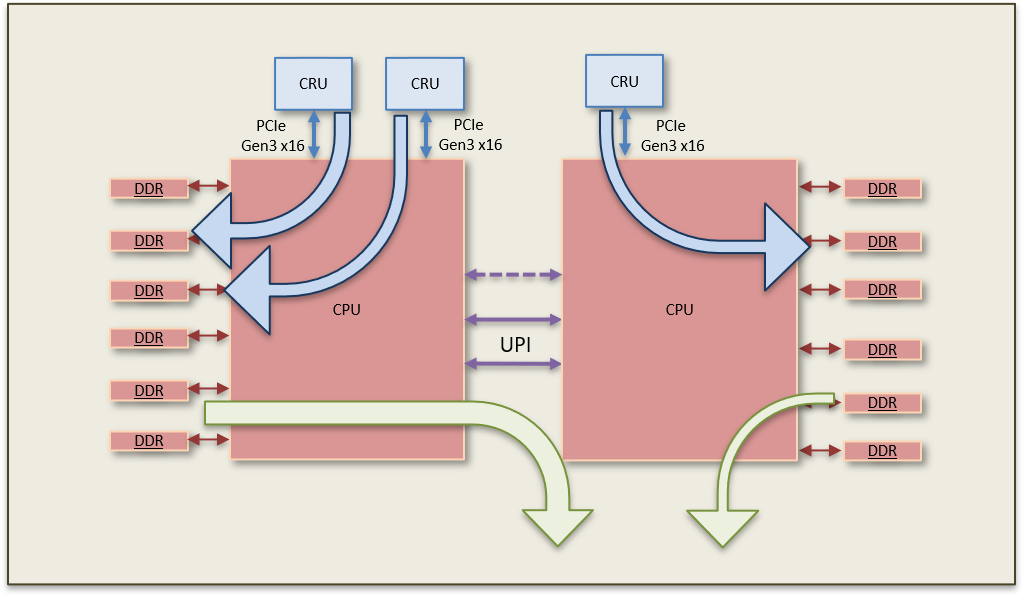
\includegraphics [width=100mm] {o2_flp/Readout_dataflows.png}
\caption{Simultaneous dataflows inside the FLP from the CRUs to the DDR memories and from the memory to the Infiniband network to the EPN farm.}
\label{fig_RO}
\end{figure}
%
 
%
%>>>>>>>>>>>>>>>>>>>>>>>>>>>>>>>>>>>>>>>>>>>>>>>>>>>>>>>>>> The data quality control 
%
\subsubsection{The data quality control}
The online execution of the calibration and the reconstruction and the replacement of the raw input data by reconstructed data, make the need for a reliable data Quality Control (QC) even more essential than usual. Its main motivations are to identify and help overcome problems during data taking and check that the data processing behaves as expected, thus ensuring good quality data for physics analyses.

The $O^2$  QC system \cite{ref_QC} is a distributed software as shown in Fig.\ref{fig_QC}.
    Data samples are selected following a pseudo-random sampling and configurable policies at key points in the data-flow and are dispatched to local (on the FLPs and the EPNs) or remote (on QC servers) QC tasks executing detector-specific algorithms. Their results are published as QC Objects, typically ROOT~\cite{ref_ROOT} histograms. The results of the QC tasks running in parallel on many nodes are assembled by the mergers.  
    Traditional or machine-learning-based checkers evaluate the quality of the objects and produce QC qualities. Finally the QC Objects and the Qualities are stored in the QC repository. This database uses the same technology as the Calibration and Condition DataBase of ALICE $O^2$. The Post-processing component encompasses asynchronous tasks such as correlation and trending of data derived from QC Objects and Qualities and triggered periodically, manually or on certain events (e.g. start of run or end of fill).
    QC and Quality Objects are accessible to shifters and experts through a web-based QC GUI.
%\end{itemize}
%
\begin{figure}[!h]
\centering
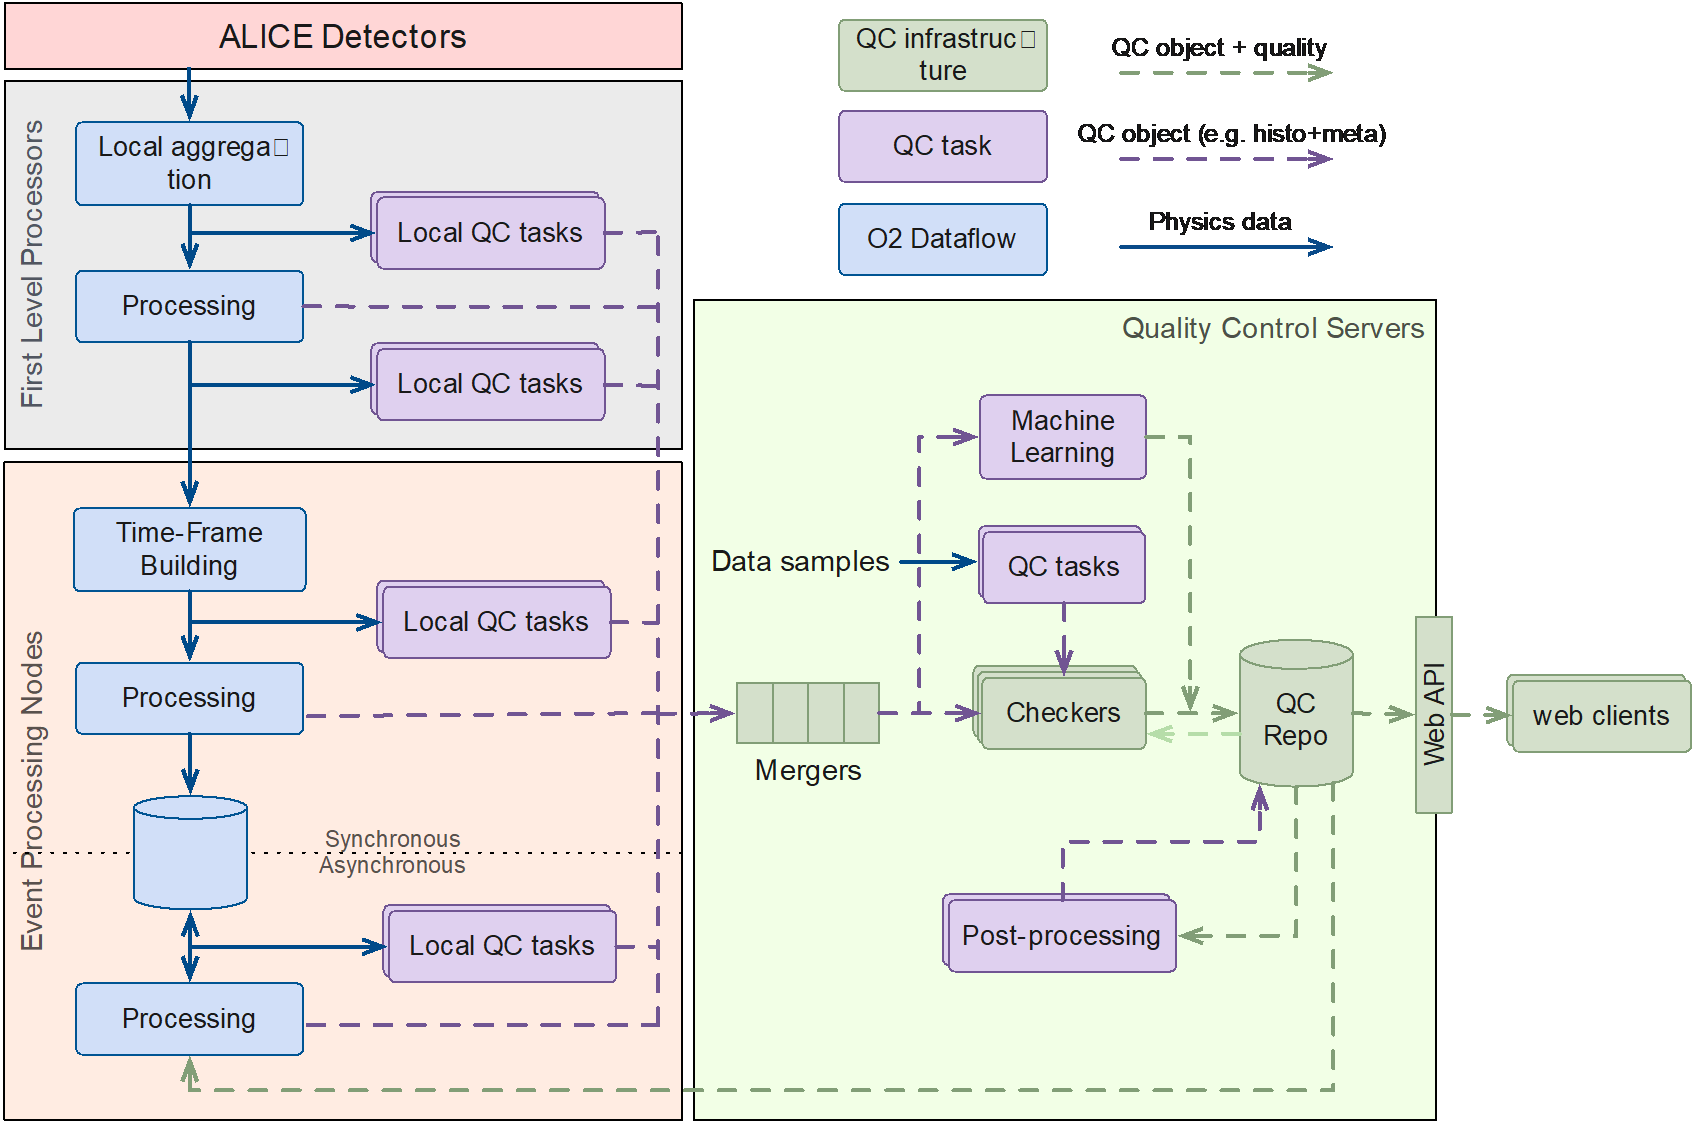
\includegraphics [width=100mm] {o2_flp/QC_Design.png}
\caption{$O^2$ Quality Control design.}
\label{fig_QC}
\end{figure}
%
%>>>>>>>>>>>>>>>>>>>>>>>>>>>>>>>>>>>>>>>>>>>>>>>>>>>>>>>>>> The services 
%
\subsubsection{The services}
%
%>>>>>>>>>>>>>>>>>>>>>>>>>>>>>>>>>>>>>>>>>>>>>>>>>>>>>>>>>> WebUI
\paragraph {Web User Interface framework}
Overview
The Web User Interface (Web UI) framework provides the core functionalities and building blocks to easily create rich web applications.
The server side features REST and WebSocket API, the authentication via CERN single sign-on and the authorisation using CERN e-groups.
The client-side features user interface Cascading Style Sheet building blocks, asynchronous data fetching (Ajax) and bi-directional socket (WebSockets).

%>>>>>>>>>>>>>>>>>>>>>>>>>>>>>>>>>>>>>>>>>>>>>>>>>>>>>>>>>> Control and configuration 
%
\paragraph{Control and configuration}
The ALICE Experiment Control System (AliECS) \cite{ref_aliecs} integrates the experiment control and configuration, the FLP farm control and a high-level control interface to the $O^2$/EPN cluster as shown in Fig~\ref{fig_aliecs}. It implements a distributed state machine to represent the aggregated state of the constituent $O^2$ processes of a data-driven workflow. Furthermore, it allows reconfiguration of running processes and simultaneous operation of multiple worflows, with easy reallocation of resources among workflows. Finally, it reacts promptly to inputs, handling events from the user, the LHC, the trigger system, the DCS, and the cluster itself with a high degree of autonomy. 

AliECS uses FairMQ, part of ALFA \cite{ref_alfa}, which is the common $O^2$ transport layer for physics data.   
Apache Mesos~\cite{ref_mesos} is a cluster resource management system, which facilitates the management of O2/FLP components, resources and tasks inside the O2/FLP facility, 
effectively enabling the developer to program against the datacenter (i.e., the O2/FLP facility at LHC Point 2) as if it was a single pool of resources. 

AliECS interfaces with Consul~\cite{ref_consul}, a key-value store which acts as the system’s configuration repository. The design also includes interfacing with information sources from the LHC, 
the trigger system, and the DCS. Once acquired by the AliECS core, configuration information is processed into an in-memory hierarchical key-value store, and from there it is
fed into a template system in order to generate task deployment and configuration structures.

Most components of AliECS are written in Go~\cite{ref_go}, a statically typed general purpose programming language in the tradition of C, which is particularly suitable for distributed system development because of its advanced synchronization and threading facilities.

\begin{figure}[!h]
\centering
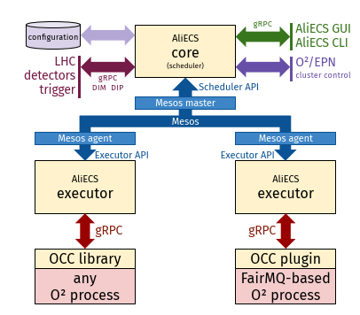
\includegraphics [width=100mm] {o2_flp/AliECS_Design.png}
\caption{AliECS design.}
\label{fig_aliecs}
\end{figure}

%
%>>>>>>>>>>>>>>>>>>>>>>>>>>>>>>>>>>>>>>>>>>>>>>>>>>>>>>>>>> Monitoring 
%
\paragraph{Monitoring}
The monitoring subsystem \cite{ref_monitor1, ref_monitor2} provides a complete overview of the overall system health, detects performance degradation and component failures by collecting, processing, storing and visualising values from hardware and software sensors and probes. As presented in Fig.~\ref{fig_monitoring}, metrics are sent to the system from both Telegraf \cite{ref_telegraf} (for system metrics) and the C++ monitoring library (via Telegraf, for application metrics). These metrics are processed in an Apache Kafka \cite{ref_Kafka} cluster and later written to InfluxDB \cite{ref_influxdb} time-series database for permanent storage.

InfluxDB time-series database supports downsampling which decreases the value resolution over time bringing down the total database size. It is planned to keep high resolution metrics for several days. After that time metrics will be downsampled in order to decrease the number of points and store them until the end of the calendar year. 

The system includes a data visualisation interface based on Grafana \cite{ref_grafana} and channels to email or mattermost for alarms and reporting.
\begin{figure}[!h]
\centering
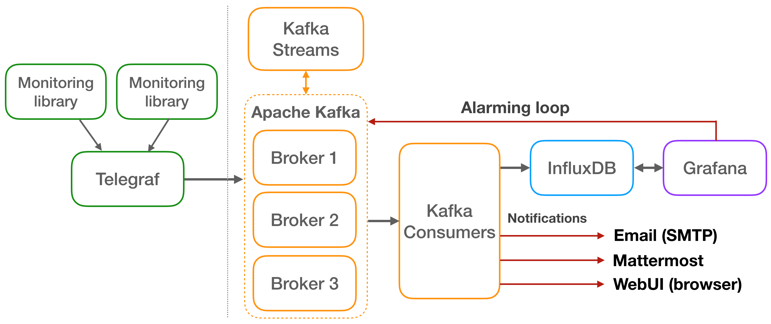
\includegraphics [width=100mm] {o2_flp/Monitoring_Design.png}
\caption{The $O^2$ computing system monitoring design.}
\label{fig_monitoring}
\end{figure}

%
%>>>>>>>>>>>>>>>>>>>>>>>>>>>>>>>>>>>>>>>>>>>>>>>>>>>>>>>>>> Logging 
%
\paragraph{Logging}
The logging system has been adapted from the ALICE Run 2 DAQ software \cite{ref_logging}. A new web-based user interface has been developed in addition to the existing GUIs.
%
%>>>>>>>>>>>>>>>>>>>>>>>>>>>>>>>>>>>>>>>>>>>>>>>>>>>>>>>>>> Bookkeeping 
%
\paragraph{Bookkeeping}
A new bookkeeping system called Jiskefet \cite{ref_bookkeeping} has been developed. It unifies two functionalities: gathering, storing and presenting metadata associated with the operations of the ALICE experiment and tracking the asynchronous processing of the physics data. The front end is based on the WebUI framework like the other applications and is adaptive to various clients such as tablets, mobile devices and other screens. The back end includes an OpenAPI specification based REST API and a relational database.


\subsection{EPN (Volker; 3p.)}
\subsection{Grid computing (Andreas; 3 p.)}


\section{Conclusions (Werner, Alex, Marco, Jochen; 5 p.)}
\subsection{Prospects for Run 3 + 4 (expected performance)}


\cleardoublepage
%%%%% acknowledgements - handled by EB chairs
\newenvironment{acknowledgement}{\relax}{\relax}
\begin{acknowledgement}
\section*{Acknowledgements}
% add specific acknowledgements here
% ...but please don't remove the line below: funding agencies
% will be acknowledged with a custom tex file handled by EB chairs after Collab Round 2
%\input{acknowledgements.tex}
\end{acknowledgement}

%%%%%%%% Bibliography
\bibliographystyle{utphys}   % Remember we use title in the biblio
\bibliography{bibliography}
%\input {bibliography.tex}

%%%%%%%%%%%%%%%%%%%%%%%%%%%%%%%%
% Appendices: yours (if any) + authorlist
%%%%%%%%%%%%%%%%%%%%%%%%%%%%%%%%
\newpage
\appendix

%
%\input{} % put your appendices here (if any)
%

%%%%% Authorlist - please do not touch: handled by EB chairs
\section{The ALICE Collaboration}
\label{app:collab}
%\input{authorlist-preprint.tex}
\end{document}
